\chapter{Ergebnisse}
\section{Klassifizierung zwischen Tumor und no Tumor}
\subsection{Hyperparameter}
Um die Hyperparameter zu ermitteln, werden die fünf Trainingsdurchläufen (Runs) mit den niedrigsten Validation Loss betrachtet.
In der Abbildung \ref{fig:val_loss notu-tu} wird der Verlauf des validation loss dargestellt.
\begin{figure}[H]
  \centering
  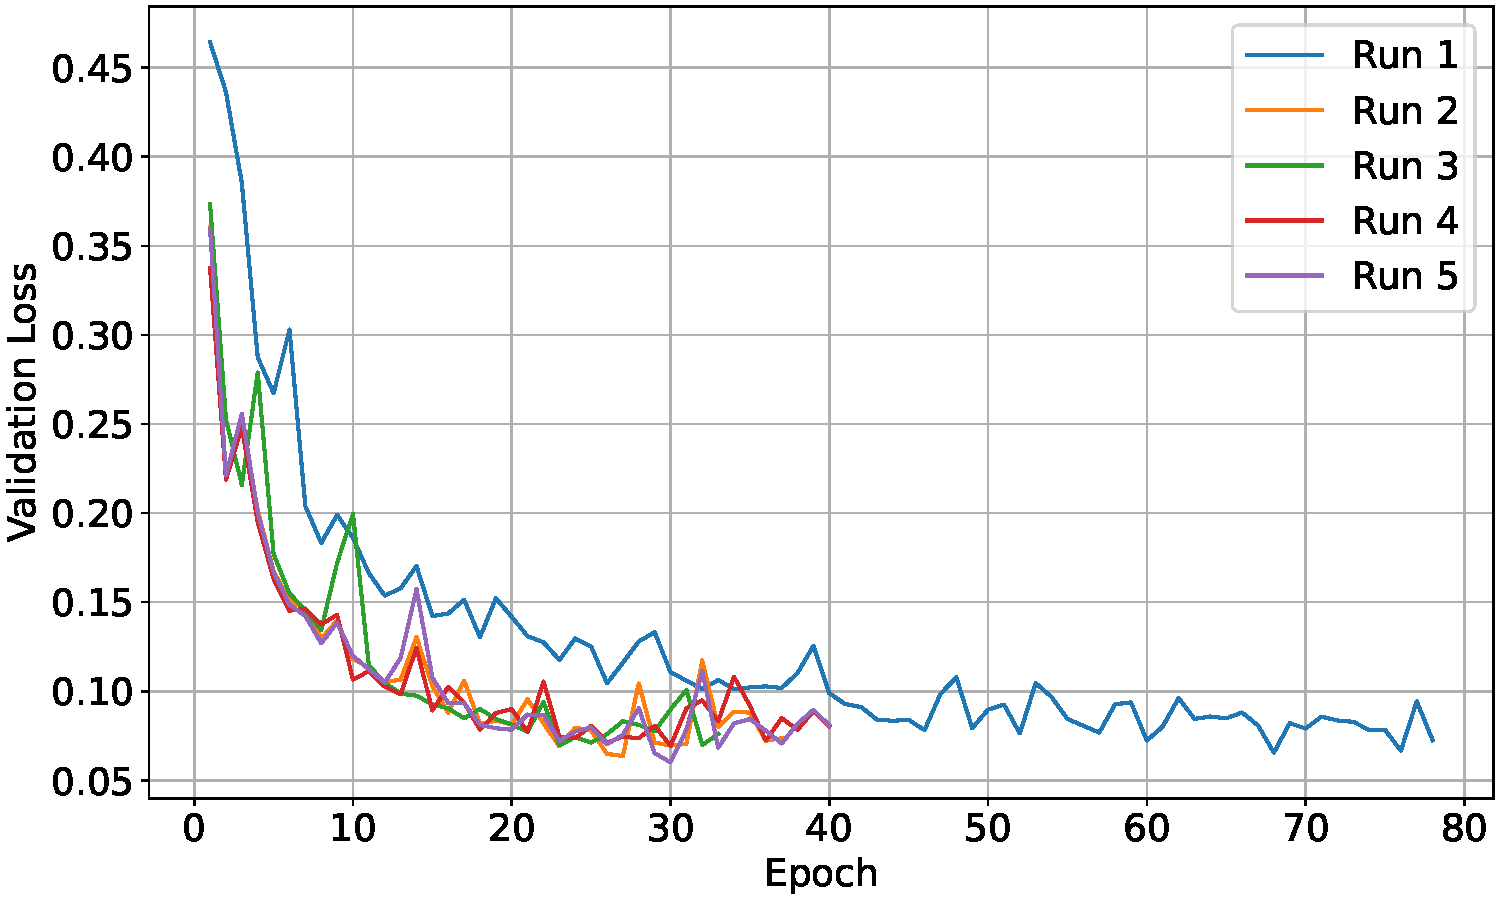
\includegraphics[scale=0.4]{plots/Val_loss_noTu_Tu.pdf}
  \caption{Verlauf des validation loss bei der Verwendung verschiedener Hyperparameter.}
  \label{fig:val_loss notu-tu}
\end{figure}
\vspace{-2em}
Die verwendeten Werte der Hyperparameter für diese fünf Runs, sowie die aufgenommene Accuracy, Sensitivity und Specificity der Validierungsdaten,
werden in der Tabelle \ref{tab:hyperp notu-tu} aufgezeigt.
\begin{table}[H]
    \centering
    \resizebox{\textwidth}{!}{%
        \begin{tabular}{cccccccc}
            \toprule
            Runs & Batch Größe & Lernrate & Dropout & validation loss & Accuracy/$\%$ & Sensitivity & Specificity \\
            \midrule
            1 & 128 & 0.005  & 0.55 & 0.072539 & 97.53231 & 0.97967 & 0.96774 \\
            2 & 128 & 0.0005 & 0.5  & 0.073672 & 98.00235 & 0.98706 & 0.96774 \\
            3 & 16  & 0.0001 & 0.5  & 0.076007 & 97.88484 & 0.97597 & 0.98387 \\
            4 & 128 & 0.0005 & 0.4  & 0.080399 & 97.76733 & 0.97782 & 0.97742 \\
            5 & 128 & 0.0005 & 0.5  & 0.080853 & 97.64982 & 0.98706 & 0.95806 \\
            \bottomrule
        \end{tabular}
    }
  \caption{Die fünf Runs mit dem niedrigsten validation loss sowie deren verwendete Hyperparameter und aufgezeichnete Metriken.}
  \label{tab:hyperp notu-tu}
\end{table}
Die Werte der Accuracy, Sensitivity und Specificity liegen dicht bei einander und schwanken nur geringfügig.
Da die Ergebnisse der Validierung konstant sind, werden für die weiteren Trainingsdurchläufen die Hyperparameter des Runs 1 verwendet. 

\subsection{Reduzierung der Trainingsdaten}

Das Netzwerk wurde mit unterschiedlichen Datensatzgrößen trainiert und auf einen Testdatensatz angewendet, bei dem die Accuracy, Sensitivity und Specificity berechnet wurde.
Da beobachtet wurde, dass die Werte der Metriken bei 2723 gesunken sind, wurde zusätzlich das Netzwerk mit 2553, 2893 und 3234 
Training samples trainiert.
Die Mittelwerte und Standardabweichung der Metriken wurden in Abhängigkeit von den Training samples dargestellt.
Diese Ergebnisse sind in Abbildung \ref{fig:reduzierung_trainingsdaten} sowie Tabelle \ref{tab:reduzierung_trainingsdaten} zusammengefasst.
Es ist zu erkennen, dass die drei Metriken einen ähnlichen Verlauf aufweisen.
Die niedrigsten Werte werden bei 340 Training samples aufgenommen und steigen dann kontinuierlich mit der sample Anzahl an.
Ab 2042 verwendete samples zeigen die Werte der Accuracy, Sensitivity und Specificity nur noch geringe Änderungen  .
Dabei schwankt die Accuracy im Bereich zwischen 2042 und 3404 Training samples zwischen $\qty{93.1157}{\%}$ und $\qty{96.2611}{\%}$. 
Die Werte der Sensitivity variieren in diesem Bereich zwischen 0,9147 und 0,9462 und die der Specificity um \SI{0,9741}{} und \SI{0,9872}{}.
\begin{figure}[H]
  \centering
  \begin{subfigure}[b]{0.48\textwidth}
    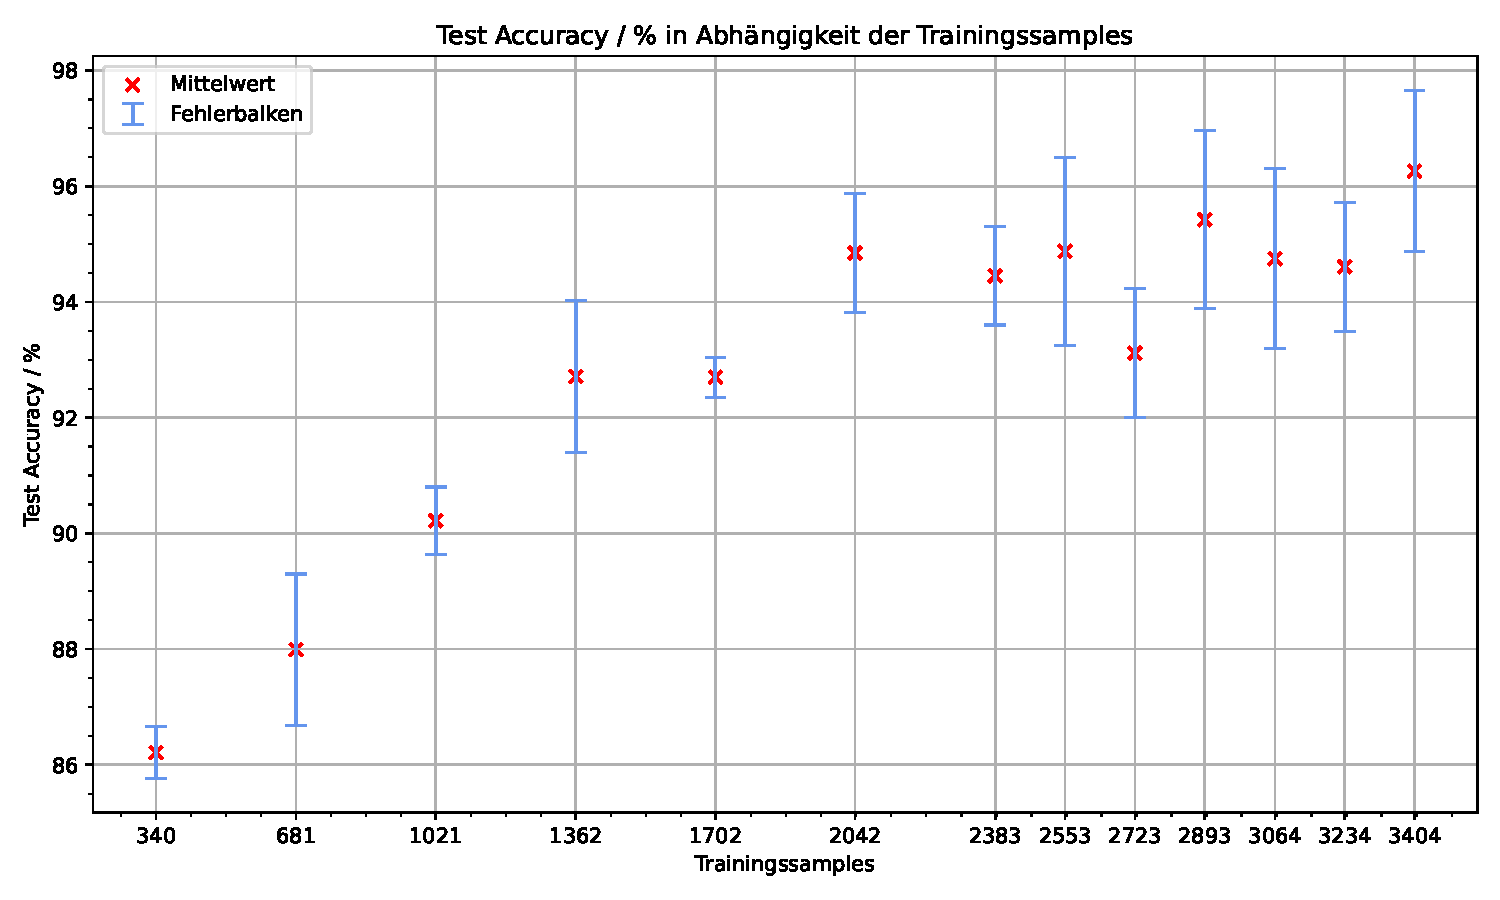
\includegraphics[width=\textwidth]{plots/2-Messungen-noTu-Tu_Accuracy_mean.pdf}
    \caption{Accuracy}
    \label{fig:reduzierung_accuracy}
  \end{subfigure}
  \begin{subfigure}[b]{0.48\textwidth}
    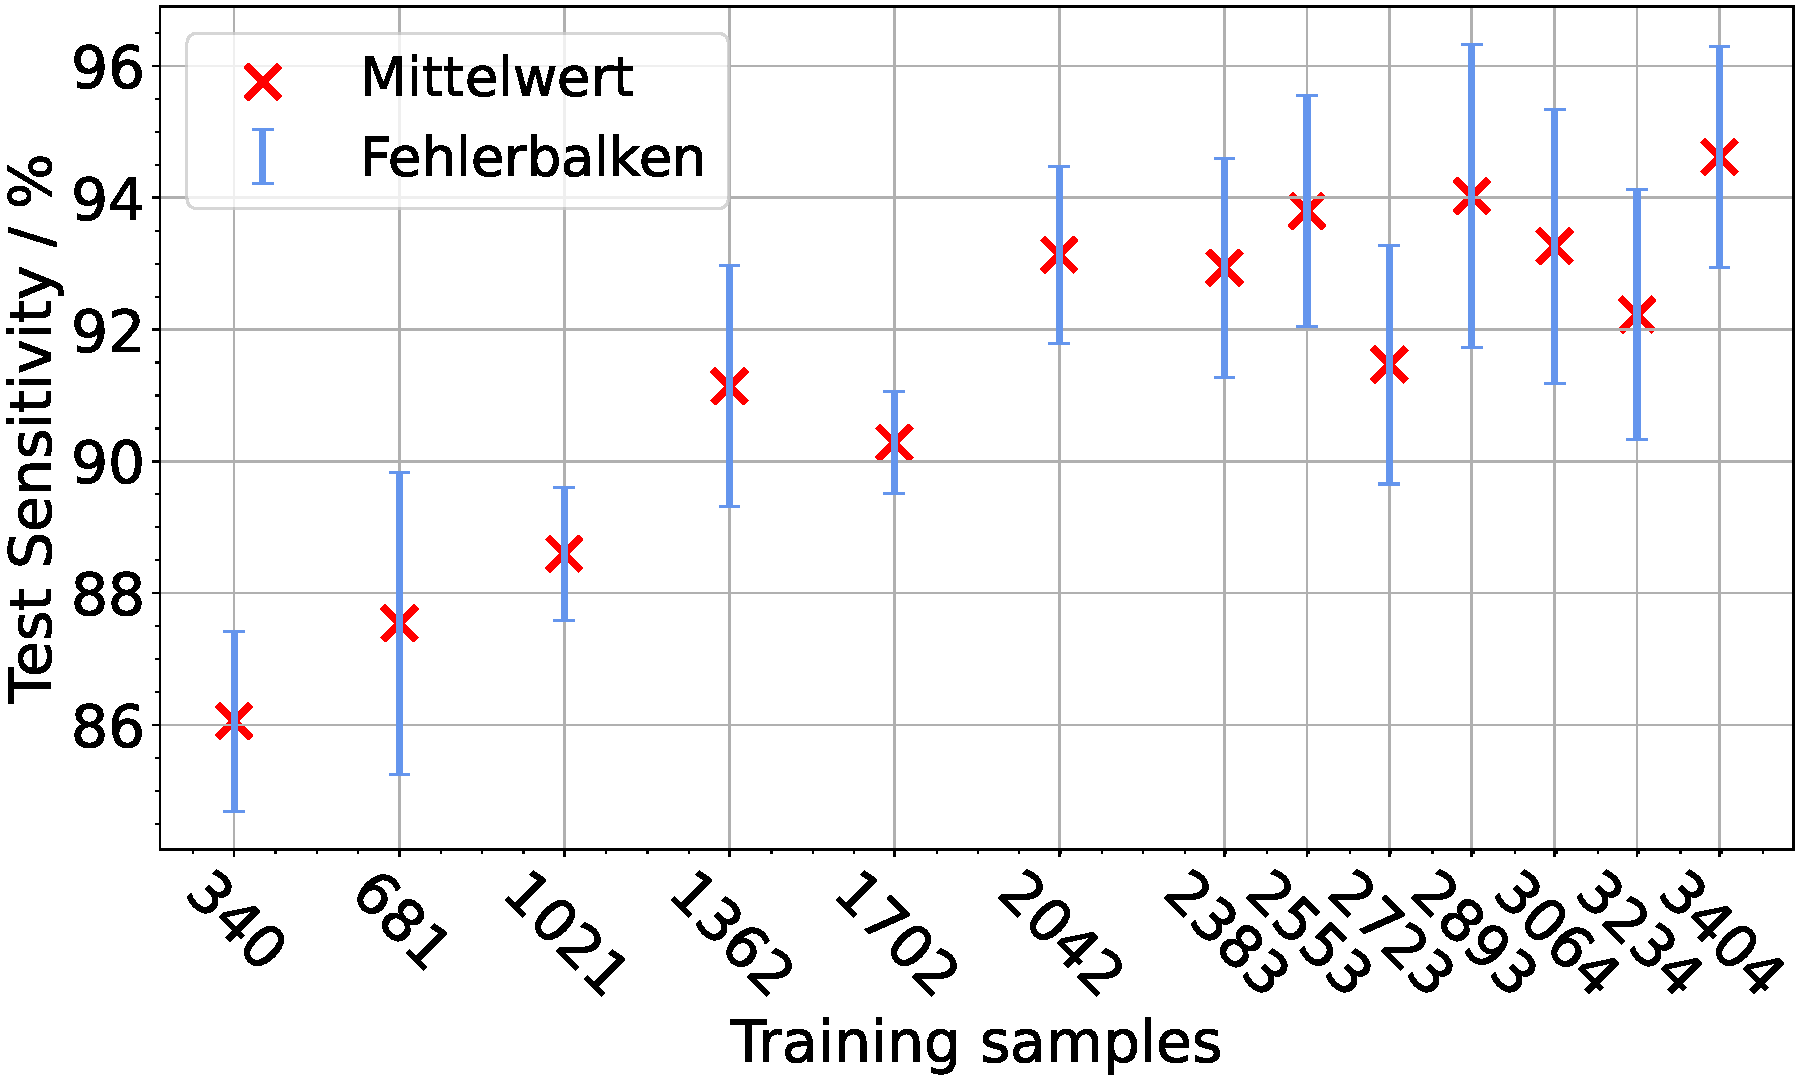
\includegraphics[width=\textwidth]{plots/2-Messungen-noTu-Tu_Sensitivity_mean.pdf}
    \caption{Sensitivity}
    \label{fig:reduzierung_sensitivity}
  \end{subfigure}
  \begin{subfigure}[b]{0.48\textwidth}
    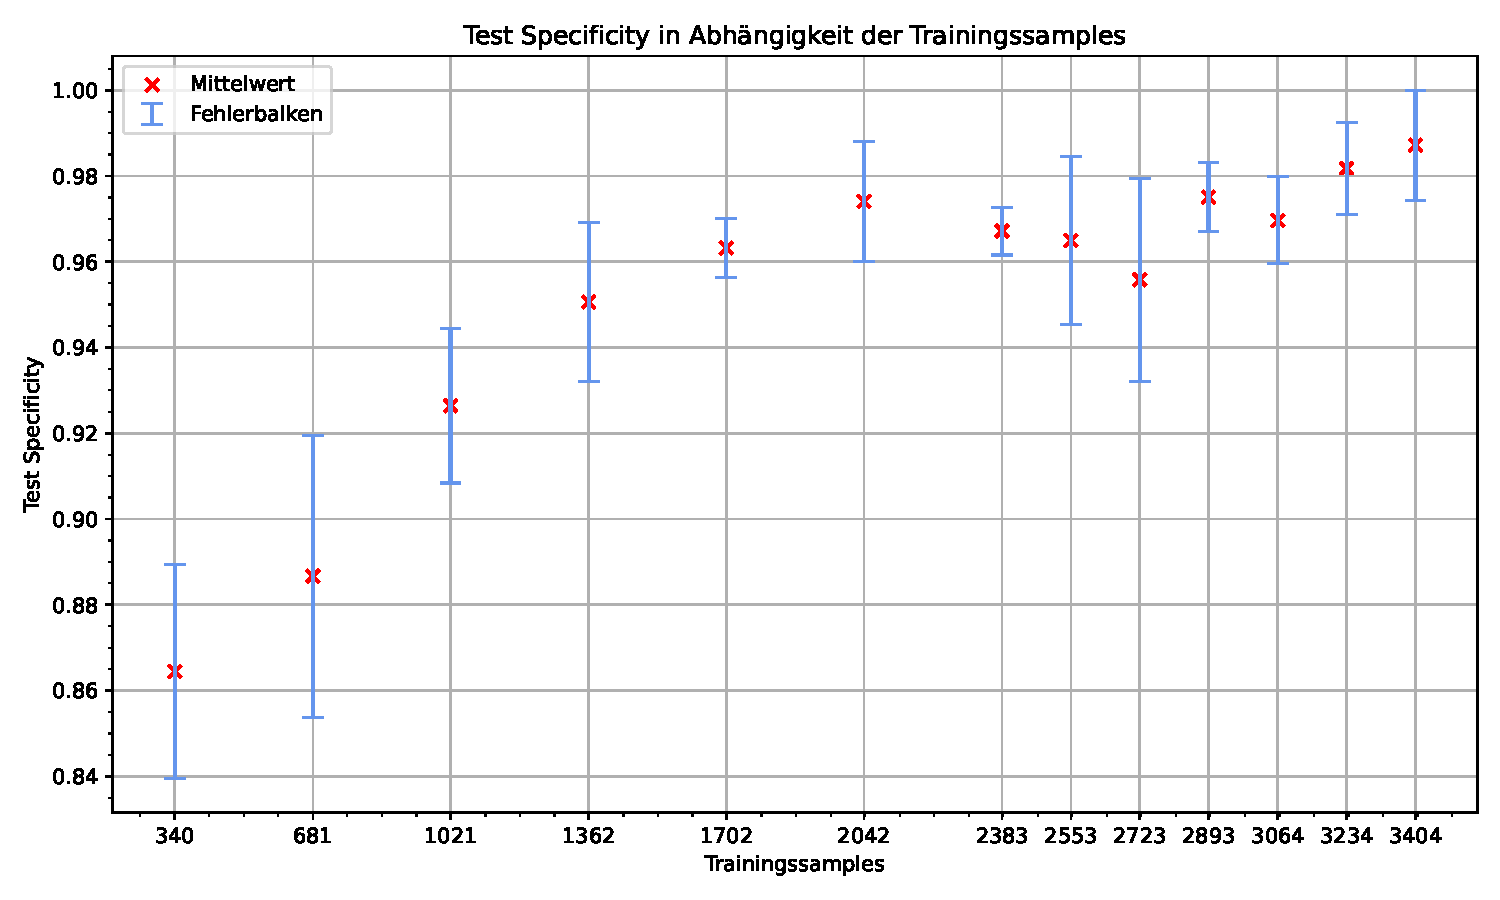
\includegraphics[width=\textwidth]{plots/2-Messungen-noTu-Tu_Specificity_mean.pdf}
    \caption{Specificity}
    \label{fig:reduzierung_specificity}
  \end{subfigure}
  \caption{Aufgenommene Metriken in Abhängigkeit der Verwendeten Trainingsdaten für die Klassifikation zwischen no Tumor und Tumor.}
  \label{fig:reduzierung_trainingsdaten}
\end{figure}
\begin{table}[H]
    \centering
    {\small
        \begin{tabular}{cccc}
            \toprule
            Training sample & Accuracy/\% & Sensitivity & Specificity\\
            \midrule
            340  & $86.2117 \pm 0.4428$ & $0.8606 \pm 0.0137 $ & $0.8644 \pm 0.0249$\\
            681  & $87.9921 \pm 1.3057$ & $0.8754 \pm 0.0229 $ & $0.8867 \pm 0.0329$\\
            1021 & $90.2176 \pm 0.5832$ & $0.8860 \pm 0.0101 $ & $0.9264 \pm 0.0180$\\
            1362 & $92.7102 \pm 1.3106$ & $0.9114 \pm 0.0183 $ & $0.9506 \pm 0.0186$\\
            1702 & $92.7003 \pm 0.3452$ & $0.9028 \pm 0.0078 $ & $0.9632 \pm 0.0068$\\
            2042 & $94.8467 \pm 1.0316$ & $0.9314 \pm 0.0134 $ & $0.9741 \pm 0.0140$\\
            2383 & $94.4510 \pm 0.8502$ & $0.9294 \pm 0.0166 $ & $0.9672 \pm 0.0056$\\
            2553 & $94.8764 \pm 1.6231$ & $0.9380 \pm 0.0175 $ & $0.9649 \pm 0.0196$\\
            2723 & $93.1157 \pm 1.1163$ & $0.9147 \pm 0.0181 $ & $0.9558 \pm 0.0237$\\
            2893 & $95.4204 \pm 1.5352$ & $0.9403 \pm 0.0230 $ & $0.9751 \pm 0.0080$\\
            3064 & $94.7478 \pm 1.5545$ & $0.9327 \pm 0.0208 $ & $0.9696 \pm 0.0102$\\
            3234 & $94.6093 \pm 1.1125$ & $0.9223 \pm 0.0190 $ & $0.9817 \pm 0.0108$\\
            3404 & $96.2611 \pm 1.3948$ & $0.9462 \pm 0.0167 $ & $0.9872 \pm 0.0128$\\ 
            \bottomrule
        \end{tabular}
    }
  \caption{Mittelwert und Standardabweichung der Metriken bei der Reduzierung der Training samples.}
  \label{tab:reduzierung_trainingsdaten}
\end{table}

\subsection{Augmentation}
Das Netzwerk wurde für verschiedene Datensatzgrößen trainiert, wobei beim Training Augmentation angewendet wurde.
Die Accuracy, Sensitivity und Specificity werden in Abhängigkeit der Training samples in Abbildung \ref{fig:augmentation_tu} abgebildet und
die dargestellten Werte werden in der Tabelle \ref{tab:augm-tunotu} aufgezeigt.
Von 340 bis 2042 Samples, steigt die Accuracy und die Specificity konstant an und geht anschließend in Plateau über.
Die Accuracy variieren innerhalb des Plateaus zwischen \SI{94.2532}{\percent} und \SI{96.4293}{\percent}. 
Die Specificity schwankt ab 2042 Training samples zwischen \SI{0.9234}{} und \SI{0.9475}{}.
Die Sensitivity steigt nur bis zu 1021 samples kontinuierlich an und bleibt bis zu 1702 Samples konstant bei ungefähr \SI{0,89}{}.
Danach steigt sie wieder an und schwankt, von 2042 bis 3404 Training samples, zwischen \SI{0.9234}{} und \SI{0.9475}{}. 
\begin{figure}[H]
  \centering
  \begin{subfigure}[b]{0.48\textwidth}
    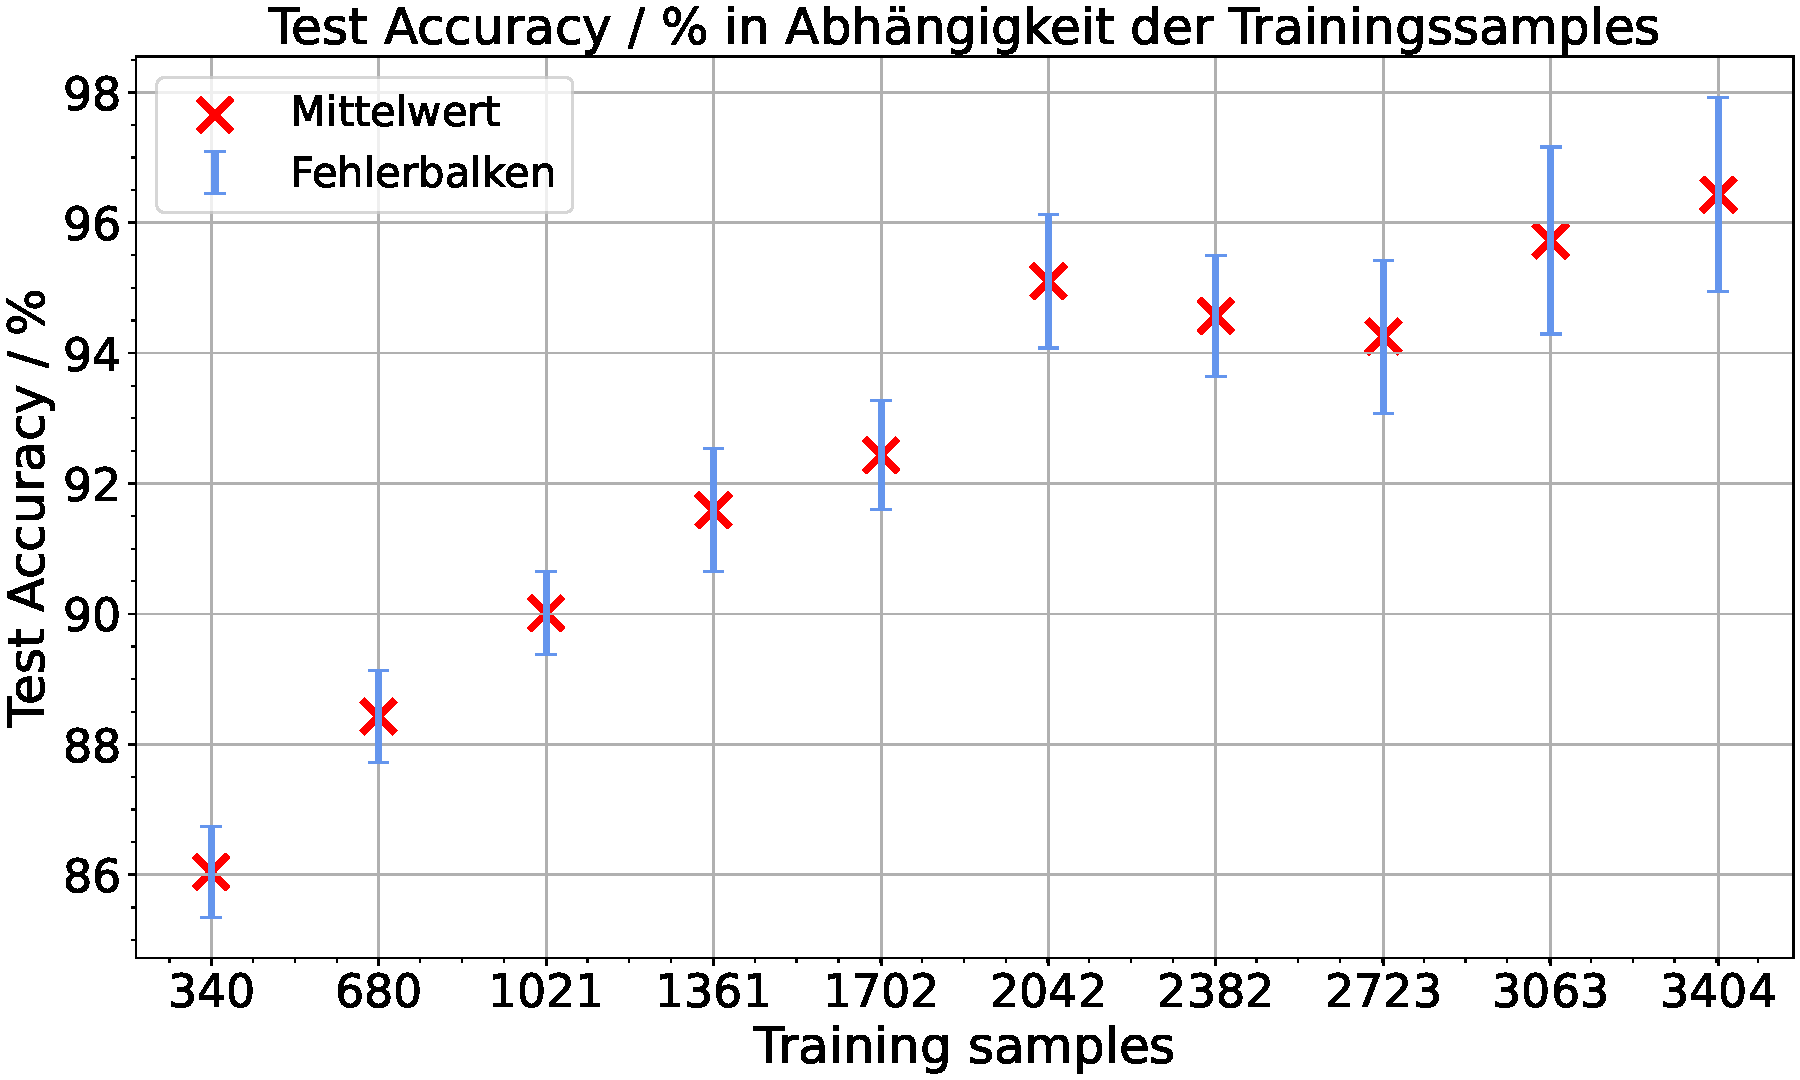
\includegraphics[width=\textwidth]{plots/Augm-Messungen-noTu-Tu_Accuracy_mean.pdf}
    \caption{Accuracy}
    \label{fig:augmentation_accuracy}
  \end{subfigure}
  \begin{subfigure}[b]{0.48\textwidth}
    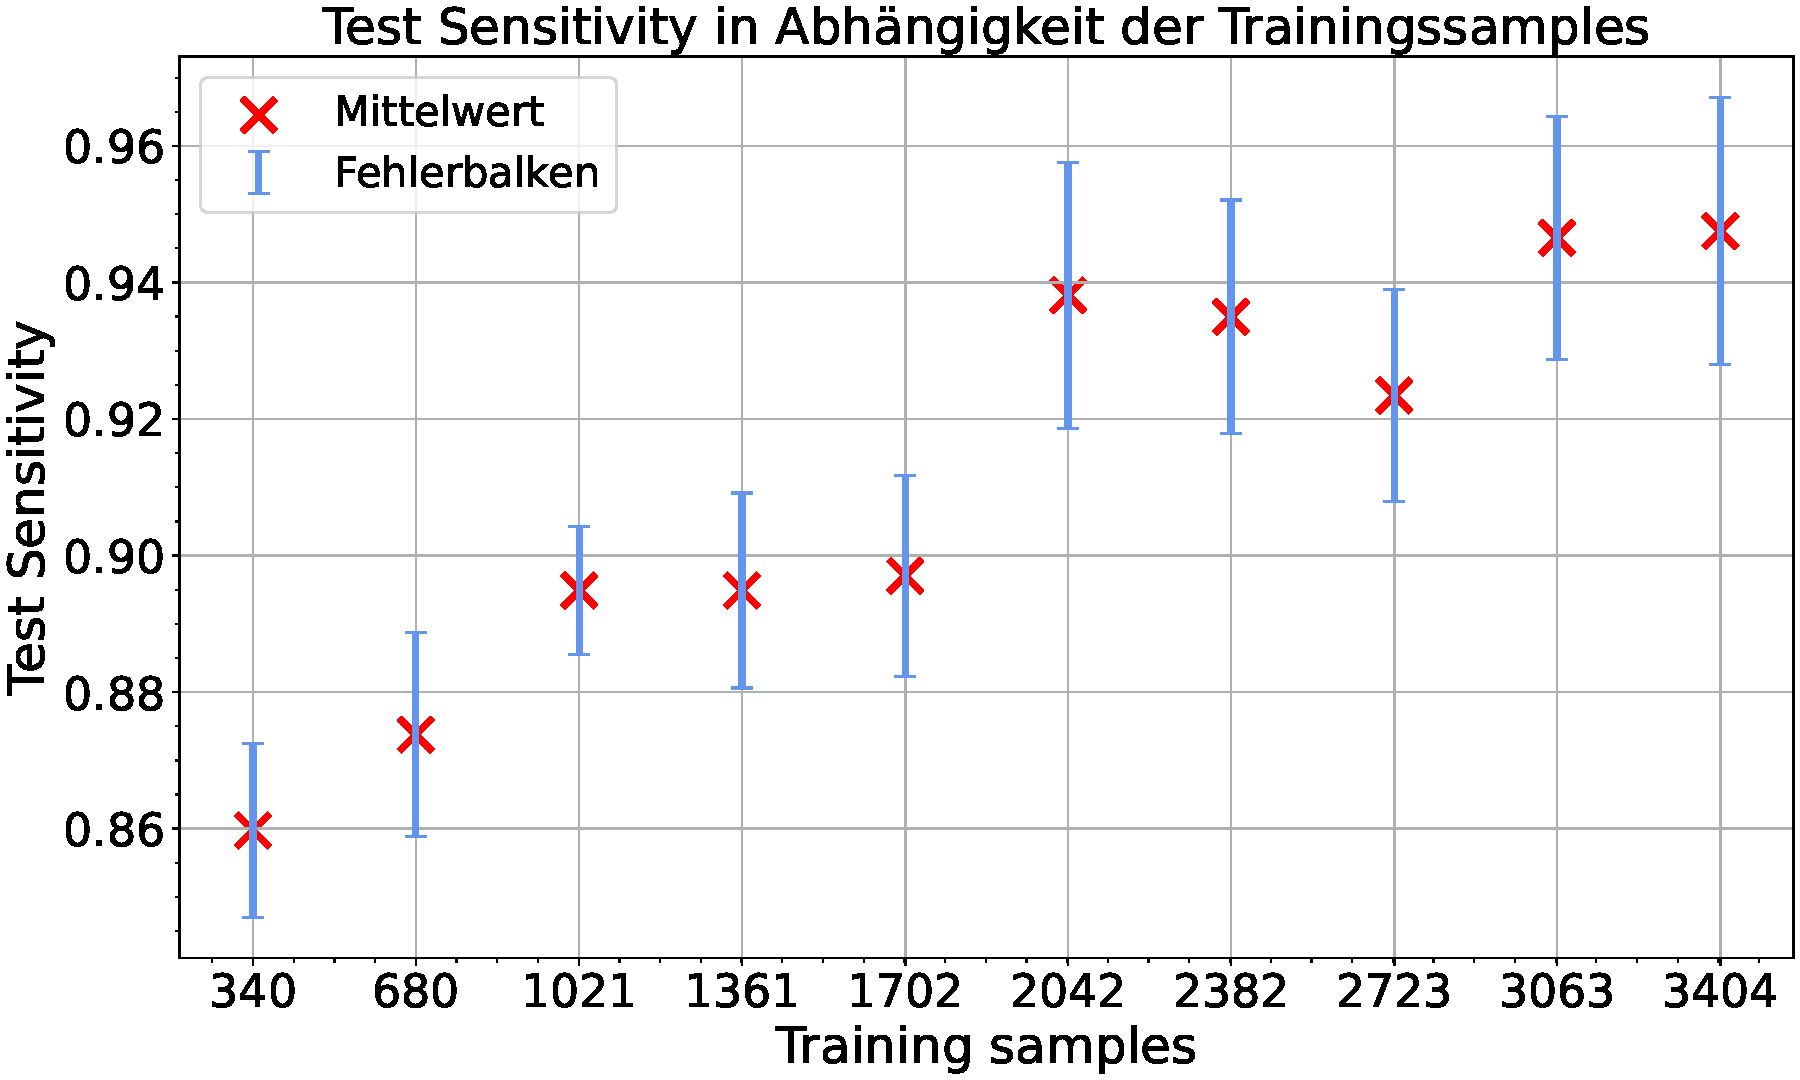
\includegraphics[width=\textwidth]{plots/Augm-Messungen-noTu-Tu_Sensitivity_mean.pdf}
    \caption{Sensitivity}
    \label{fig:augmentation_sensitivity}
  \end{subfigure}
  \begin{subfigure}[b]{0.48\textwidth}
    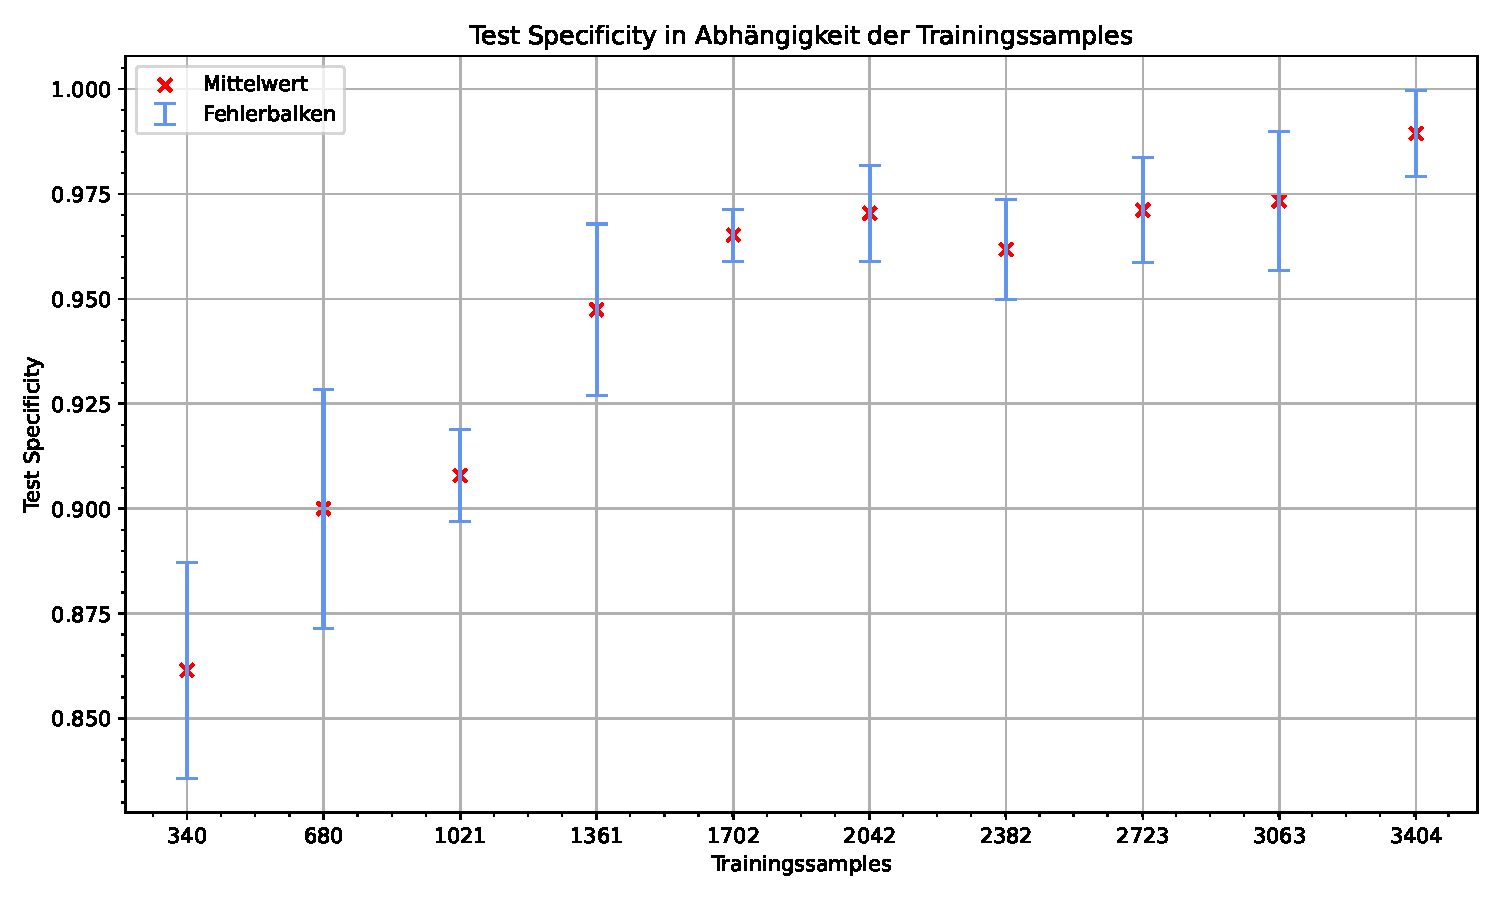
\includegraphics[width=\textwidth]{plots/Augm-Messungen-noTu-Tu_Specificity_mean.pdf}
    \caption{Specificity}
    \label{fig:augmentation_specificity}
  \end{subfigure}
  \caption{Verlauf der Metriken bei unterschiedlichen Anzahl an Training samples, unter Verwendung von Augmentation, für die Klassifikation zwischen no Tumor und Tumor.}
  \label{fig:augmentation_tu}
\end{figure}
\begin{table}[H]
    \centering
    {\small
        \begin{tabular}{cccc}
            \toprule
            Training sample & Accuracy/\% & Sensitivity & Specificity\\
            \midrule
            340  & $86.0435 \pm 0.6923$ & $0.8597 \pm 0.0127$ & $0.8615 \pm 0.0257$\\
            680  & $88.4273 \pm 0.7041$ & $0.8738 \pm 0.0150$ & $0.9000 \pm 0.0284$\\
            1021 & $90.0099 \pm 0.6376$ & $0.8949 \pm 0.0093$ & $0.9079 \pm 0.0110$\\
            1361 & $91.5925 \pm 0.9418$ & $0.8949 \pm 0.0143$ & $0.9474 \pm 0.0204$\\
            1702 & $92.4332 \pm 0.8357$ & $0.8970 \pm 0.0147$ & $0.9652 \pm 0.0062$\\
            2042 & $95.1039 \pm 1.0250$ & $0.9381 \pm 0.0195$ & $0.9704 \pm 0.0115$\\
            2382 & $94.5697 \pm 0.9296$ & $0.9350 \pm 0.0171$ & $0.9617 \pm 0.0119$\\
            2723 & $94.2532 \pm 1.1726$ & $0.9234 \pm 0.0155$ & $0.9711 \pm 0.0125$\\
            3063 & $95.7270 \pm 1.4340$ & $0.9465 \pm 0.0178$ & $0.9733 \pm 0.0166$\\
            3404 & $96.4293 \pm 1.4880$ & $0.9475 \pm 0.0195$ & $0.9894 \pm 0.0103$\\
            \bottomrule
        \end{tabular}}
  \caption{Mittelwert und Standardabweichung der Metriken bei Reduzierung der Training samples unter Verwendung von Augmentation.}
  \label{tab:augm-tunotu}
\end{table}

\subsection{Reduzierung der Tumor samples}
Für die Untersuchung der Netzwerkleistung bei Reduzierung einer Klasse, wurde die Anzahl an Tumor samples reduziert.
Der Verlauf der drei Metriken, sowie die Werte werden in der Abbildung \ref{fig:reduzierung_tumorsamples} und in der Tabelle \ref{tab:red_tu} dargestellt.
Die Accuracy steigt mit zunehmender Anzahl an samples bis zu maximal \SI{96.7458}{\percent} für 1702 Training samples.
Bei 1276 und 2128 samples sinkt sie auf ungefähr \SI{92}{\percent} ab. 
Die Sensitivity bleibt von 212 bis 851 Tumor samples konstant bei ca. \SI{0.9}{}.
Danach steigt sie leicht an und erreicht bei 1915 verwendeten Bildern einen Wert von \SI{0.9515}{}.
Auch hier sinkt bei der Verwendung aller Tumor Bilder die Sensitivity wieder ab.
Die Specificity steigt mit höherer sample Anzahl und konvergiert gegen \SI{1.0}.
Bei 212 und 1276 Tumor samples tritt eine hohe Standardabweichung für die Specificity und Accuracy auf.
Zusätzlich kommt es auch bei 2128, für die Accuracy und für die Sensitivity, zu einer große Abweichung
Bei den Klassengrößen 
In Runs bei denen 212 und 1276 Tumor samples verwendet wurden, lag die Specificity, 
sowie bei 2128 Tumor samples die Sensitivity bei 0.
\begin{figure}[H]
  \centering
  \begin{subfigure}[b]{0.48\textwidth}
    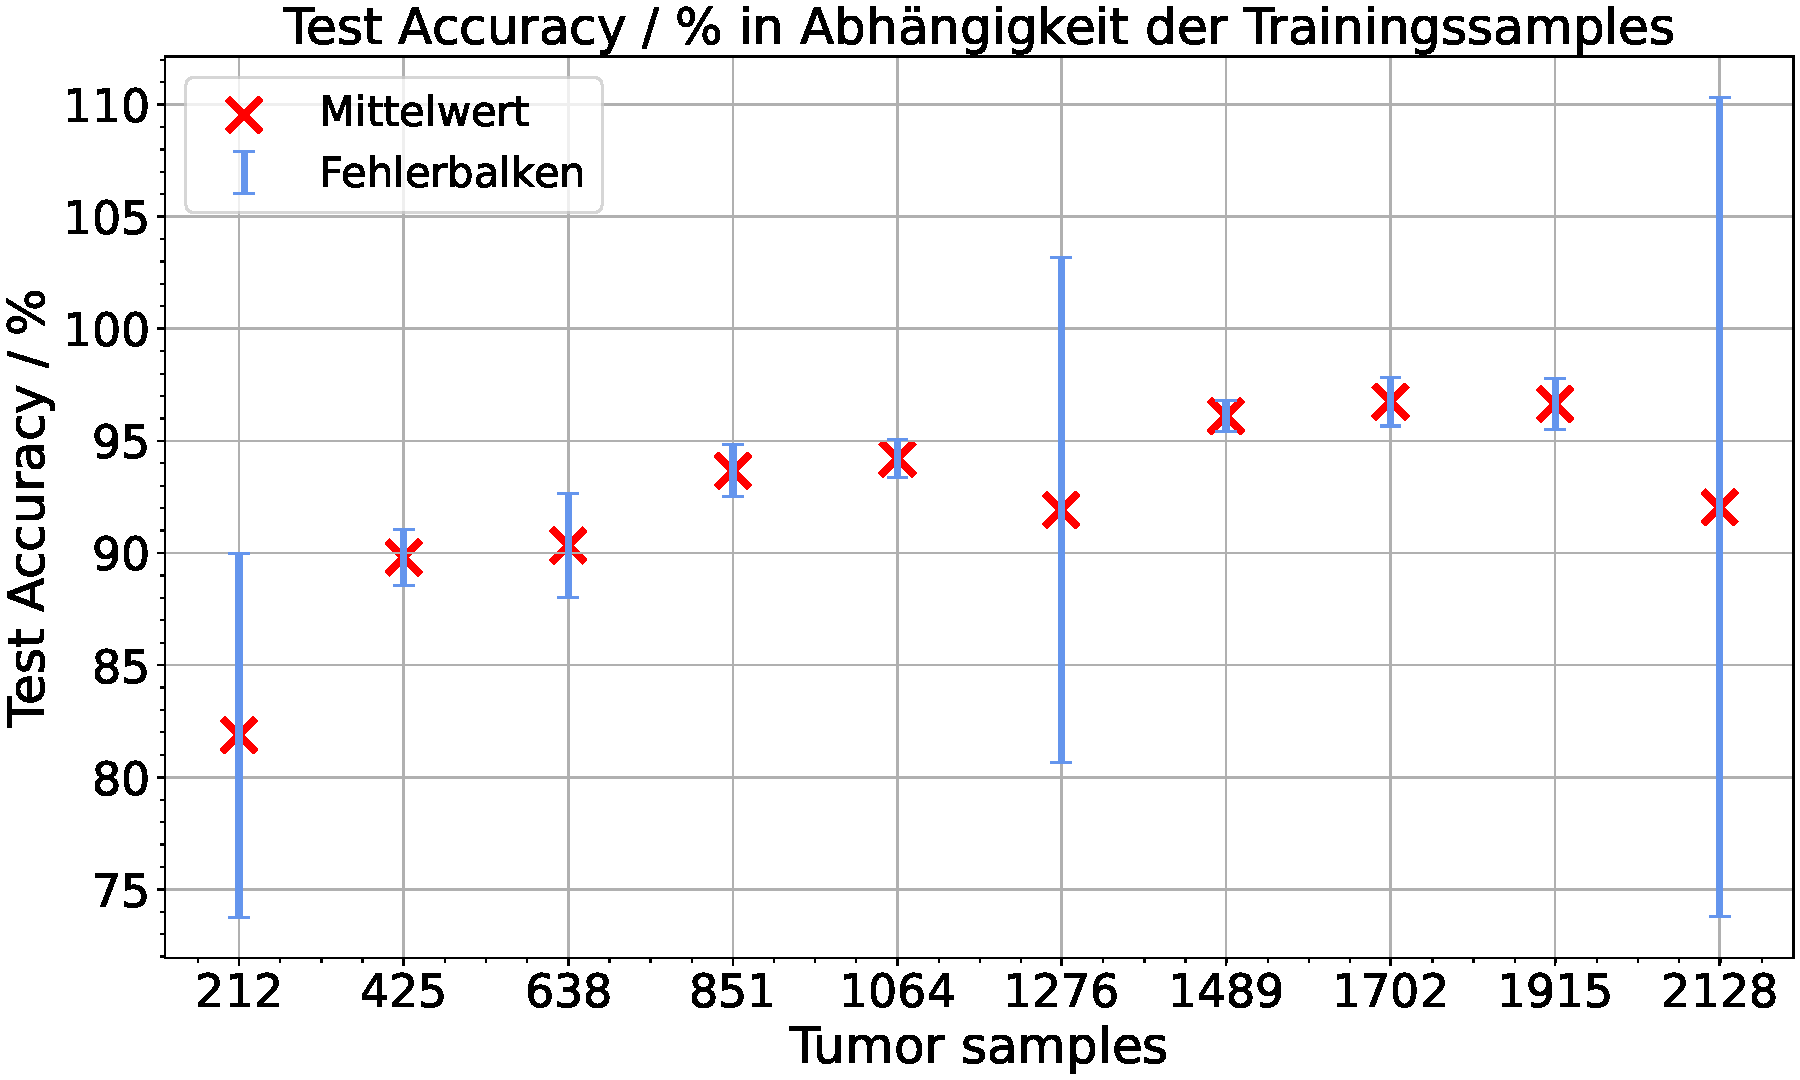
\includegraphics[width=\textwidth]{plots/neu Reduzierung-Tu + Balance_Accuracy_mean.pdf}
    \caption{Accuracy}
    \label{fig:reduzierung_tu_accuracy}
  \end{subfigure}
  \begin{subfigure}[b]{0.48\textwidth}
    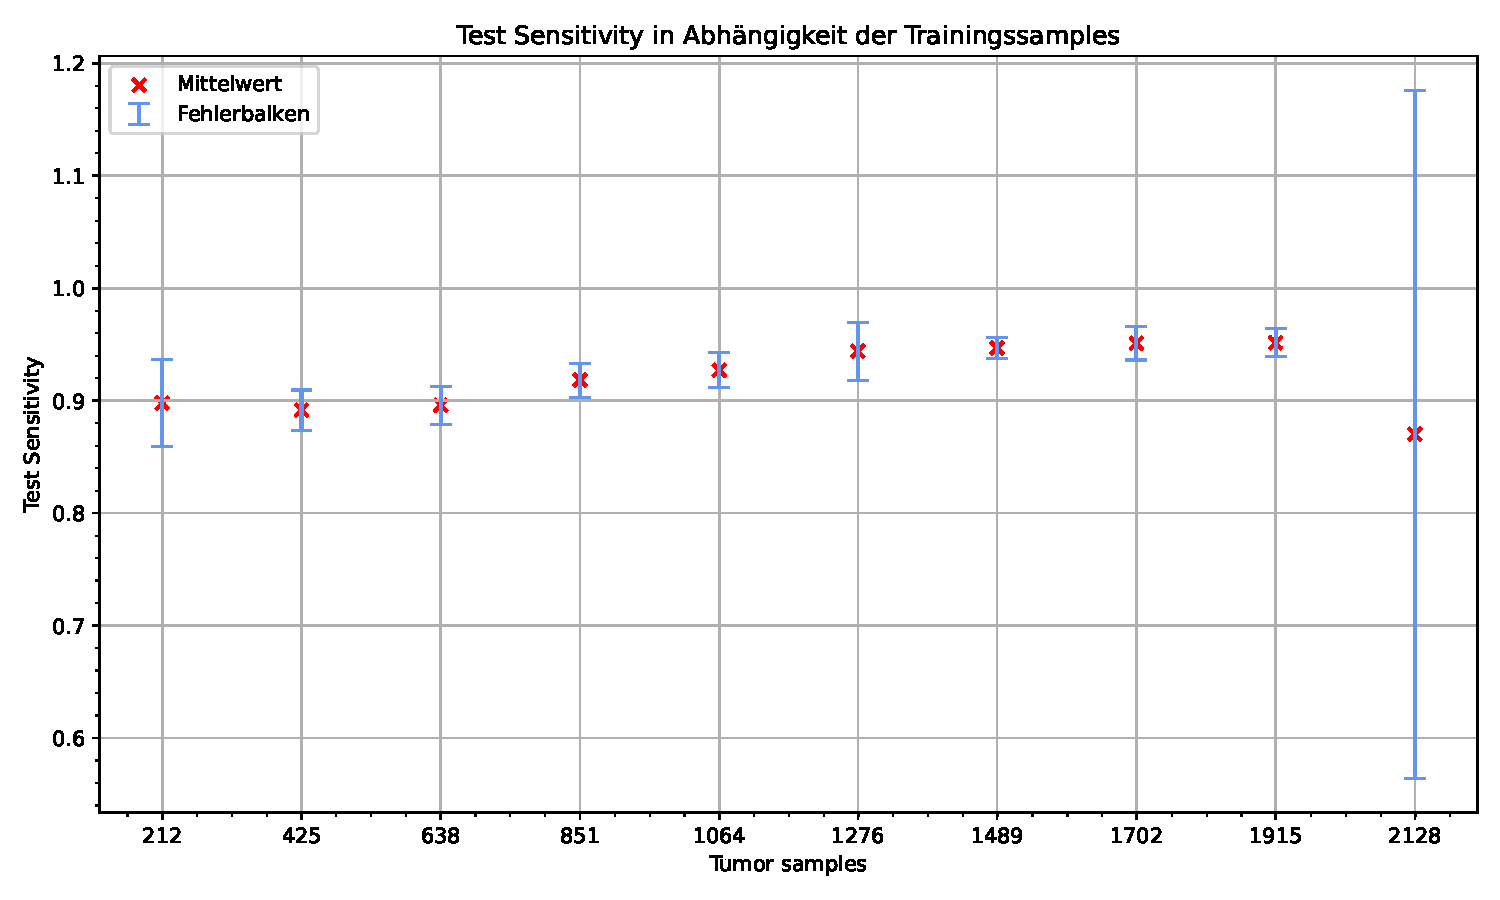
\includegraphics[width=\textwidth]{plots/neu Reduzierung-Tu + Balance_Sensitivity_mean.pdf}
    \caption{Sensitivity}
    \label{fig:reduzierung_tu_sensitivity}
  \end{subfigure}
  \begin{subfigure}[b]{0.48\textwidth}
    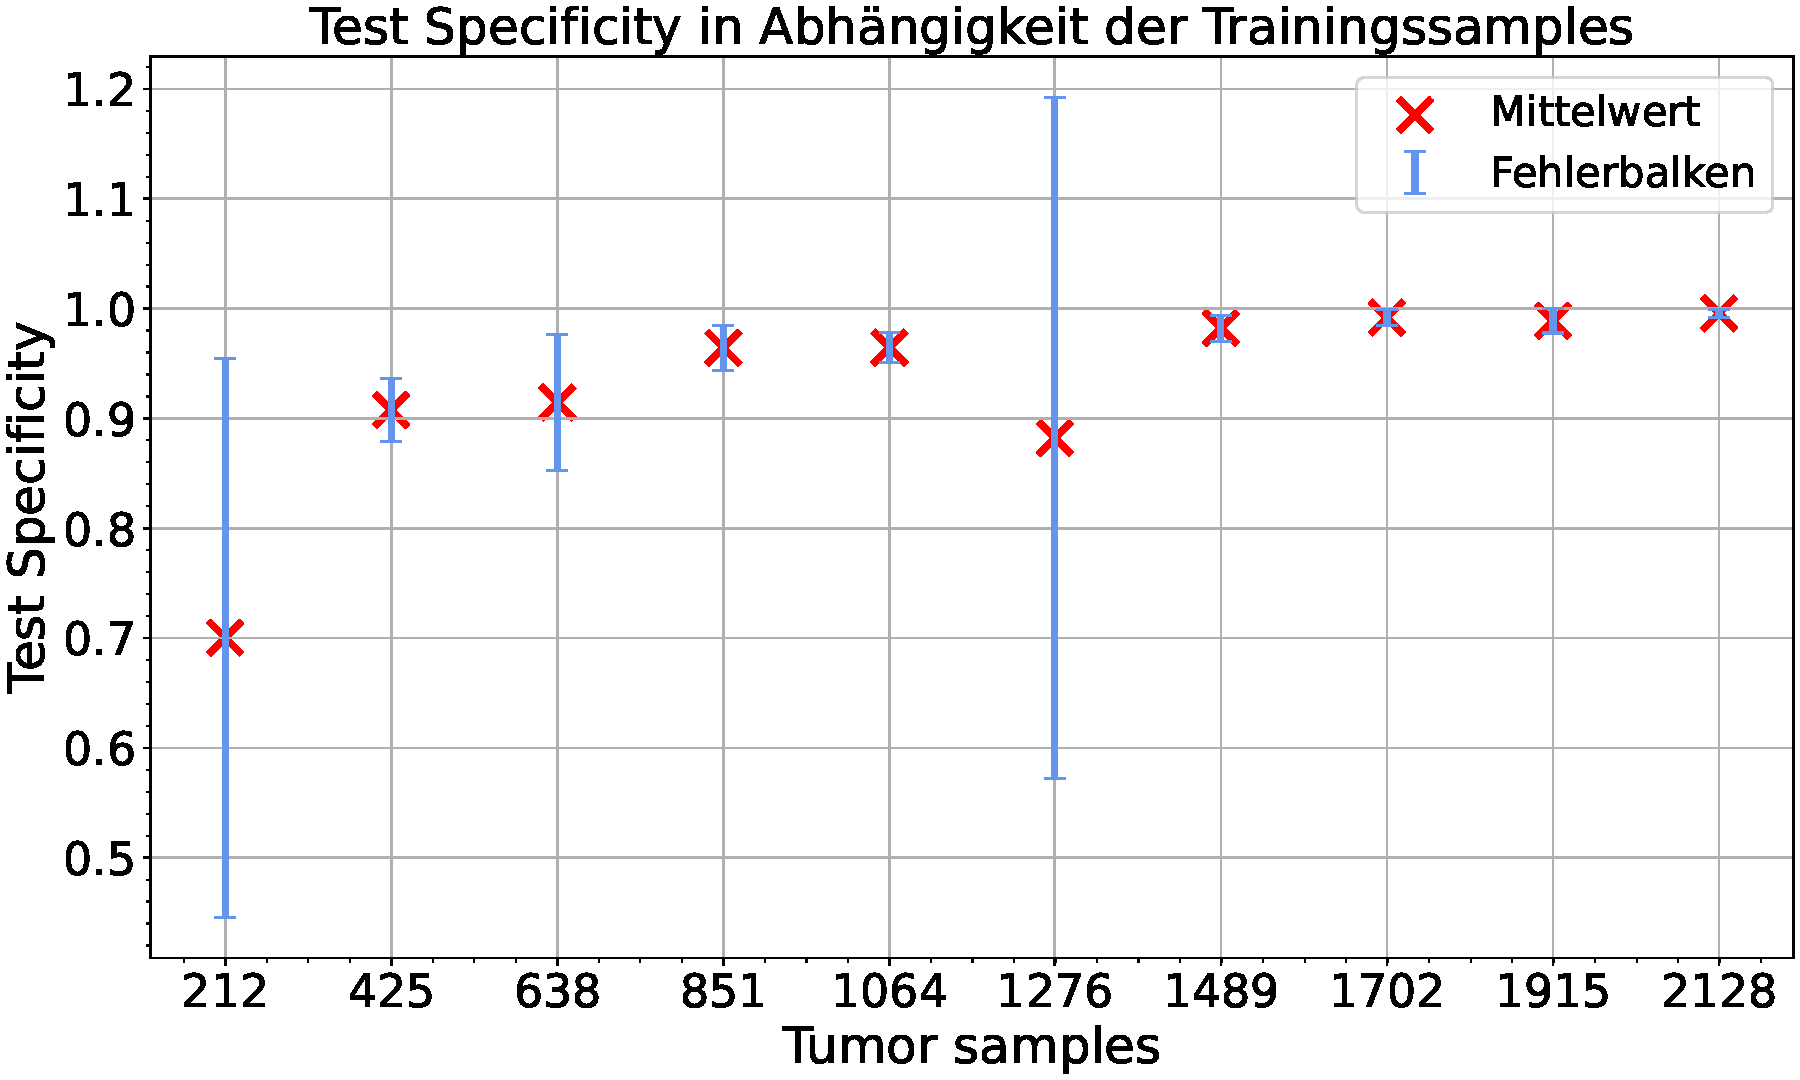
\includegraphics[width=\textwidth]{plots/neu Reduzierung-Tu + Balance_Specificity_mean.pdf}
    \caption{Specificity}
    \label{fig:reduzierung_tu_specificity}
  \end{subfigure}
  \caption{Metriken bei Reduktion der Tumor samples.}
  \label{fig:reduzierung_tumorsamples}
\end{figure}
\begin{table}[H]
    \centering
     {\small
        \begin{tabular}{cccc}
            \toprule
            Training sample & Accuracy/\% & Sensitivity & Specificity\\
            \midrule
            212  & $81.8694 \pm 8.1081$ & $0.8979 \pm 0.0389$ & $0.7002 \pm 0.2544$\\
            425  & $89.8022 \pm 1.2611$ & $0.8916 \pm 0.0179$ & $0.9077 \pm 0.0285$\\
            638  & $90.3363 \pm 2.3230$ & $0.8959 \pm 0.0170$ & $0.9146 \pm 0.0622$\\
            851  & $93.6696 \pm 1.1535$ & $0.9183 \pm 0.0151$ & $0.9642 \pm 0.0203$\\
            1064 & $94.2038 \pm 0.8486$ & $0.9271 \pm 0.0156$ & $0.9644 \pm 0.0135$\\
            1276 & $91.9189 \pm 11.273$ & $0.9441 \pm 0.0258$ & $0.8820 \pm 0.3100$\\
            1489 & $96.1029 \pm 0.6919$ & $0.9469 \pm 0.0095$ & $0.9822 \pm 0.0118$\\
            1702 & $96.7458 \pm 1.0820$ & $0.9512 \pm 0.0150$ & $0.9919 \pm 0.0069$\\
            1915 & $96.6469 \pm 1.1234$ & $0.9515 \pm 0.0124$ & $0.9889 \pm 0.0111$\\
            2128 & $92.0376 \pm 18.269$ & $0.8701 \pm 0.3058$ & $0.9956 \pm 0.0036$\\
            \bottomrule
        \end{tabular}}
  \caption{Mittelwert und Standardabweichung der Metriken bei der Reduzierung von Tumor Klasse.}
  \label{tab:red_tu}
\end{table}
%%%%%%%%%%%%%%%%%%%%%%%%%%%%%%%%%%%%%%%%%%%%%%%%%%%%%%%%%%%%%%%%%%%%%%
\section{Klassifizierung zwischen Glioma und Meningioma}
\subsection{Hyperparameter}
Für die Ermittlung der Hyperparameter werden die fünf Runs mit den niedrigsten Validation loss betrachtet.
Der Verlauf wird in der Abbildung \ref{fig:val_loss gli-men} dargestellt.
Die dazugehörigen Parameter und die Accuracy, Sensitivity und Specificity des Validierung Datensatzes werden in der Tabelle \ref{tab:hyperp-gli men} aufgelistet.
\begin{figure}[H]
  \centering
  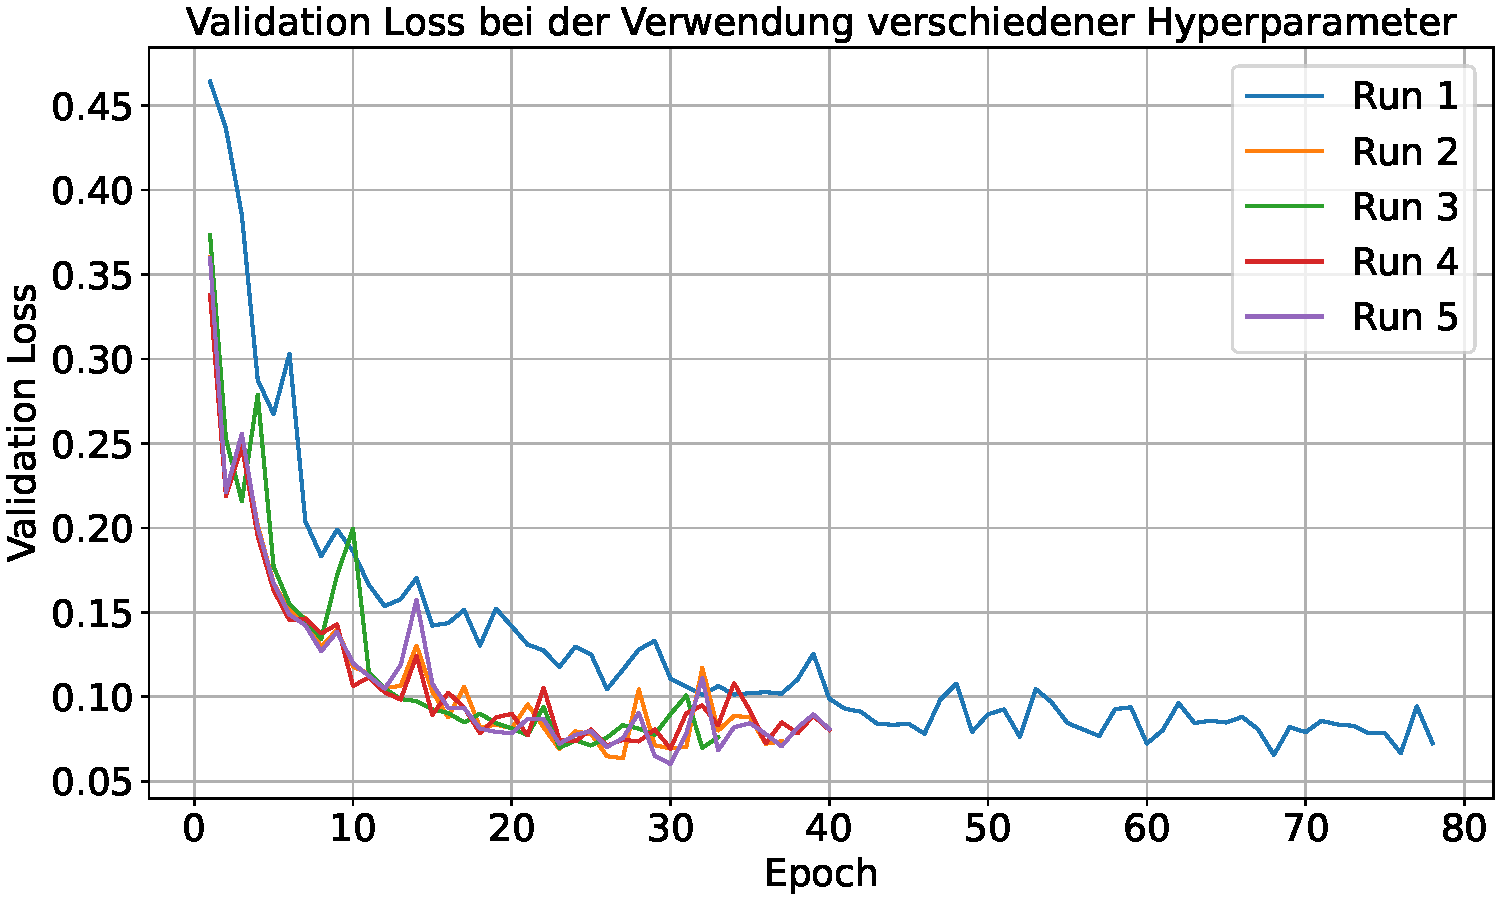
\includegraphics[scale=0.4]{plots/Val_loss_Gli_Men.pdf}
  \caption{Darstellung des validation loss bei der Verwendung verschiedener Hyperparameter.}
  \label{fig:val_loss gli-men}
\end{figure}
\begin{table}[H]
    \centering
    \resizebox{\textwidth}{!}{%
        \begin{tabular}{cccccccc}
            \toprule
            Runs & Batch Größe & Lernrate & Dropout & Validation Loss & Accuracy/$\%$ & Sensitivity & Specificity \\
            \midrule
            1 & 128 & 0.01  & 0.55 & 0.18943 & 92.29323 & 0.95402 & 0.89299 \\
            2 & 64  & 0.005 & 0.3  & 0.22499 & 93.23308 & 0.96935 & 0.89668 \\
            3 & 16  & 0.0005& 0.55 & 0.23146 & 93.98496 & 0.92720 & 0.95203 \\
            4 & 16  & 0.005 & 0.5  & 0.23453 & 92.66917 & 0.95402 & 0.90037 \\
            5 & 16  & 0.0005& 0.5  & 0.23829 & 93.42105 & 0.94253 & 0.92620 \\
            \bottomrule
        \end{tabular}
    }
  \caption{Die fünf Runs mit dem niedrigsten validation loss sowie deren verwendete Hyperparameter und aufgezeichnete Metriken.}
  \label{tab:hyperp-gli men}
\end{table}
Der erste Run besitzt zwar den niedrigsten validation loss, jedoch auch die niedrigste Accuracy und Specificity.
Der höchste Wert der Accuracy und Specificity tritt bei Run 3 auf
Aufgrund dessen werden in den folgenden Trainingsdurchläufen die Hyperparameter von Run 3 verwendet.

\subsection{Reduzierung der Trainingsdaten}
In Abbildung \ref{fig:gli-men-reduktion} ist der Verlauf der Accuracy, Sensitivity und Specificity bei der Reduktion der Training samples dargestellt.
Die dazu gehörigen Werte werden in der Tabelle \ref{tab:Red-gli-men} dargestellt.
Die drei Metriken steigen, mit zunehmender Anzahl an samples. 
Bei 851 Training samples sinken die Werte etwas, bevor sie anschließend wieder ansteigen.
Die Accuracy erhöht sich von \SI{76.4191}{\percent}, bei 231 Training samples auf \SI{92.3102}{\percent} bei 2128 Training samples.
Die Sensitivity steigt bis 1702 Training samples auf \SI{0.9186}{} an und bleibt anschließend weitgehend konstant zwischen \SI{0.9114}{} und \SI{0.9255}{}.
Die Specificity nimmt bis 1064 Training samples zu und bleibt bis 1277 konstant. 
Danach sinkt diese kurzzeitig etwas und steigt anschließend wieder an. 
Ab 1915 Training samples bleibt die Specificity stabil bei ungefähr \SI{0.92}{}.
\begin{figure}[H]
  \centering
  \begin{subfigure}[b]{0.48\textwidth}
    \centering
    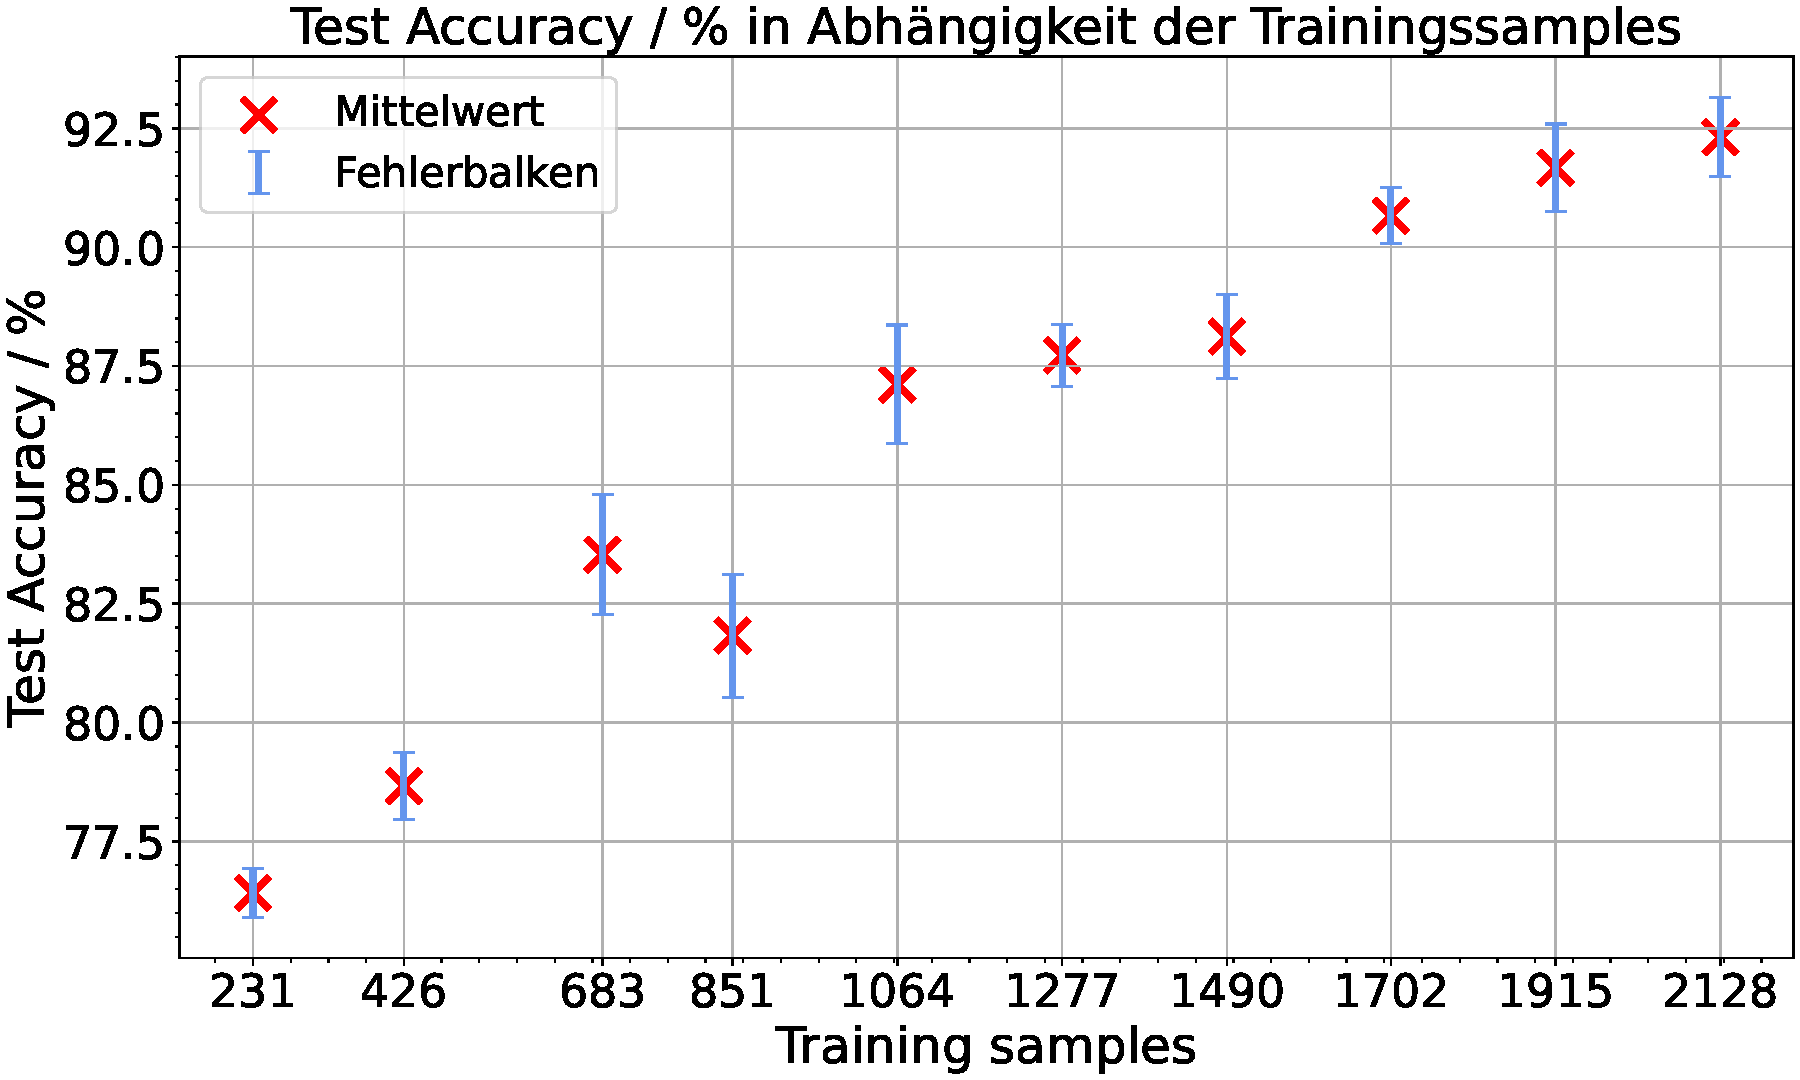
\includegraphics[width=\textwidth]{plots/3-Messungen-Gli-Men_Accuracy_mean.pdf}
    \caption{Accuracy}
    \label{fig:gli-men-acc}
  \end{subfigure}
  \begin{subfigure}[b]{0.48\textwidth}
    \centering
    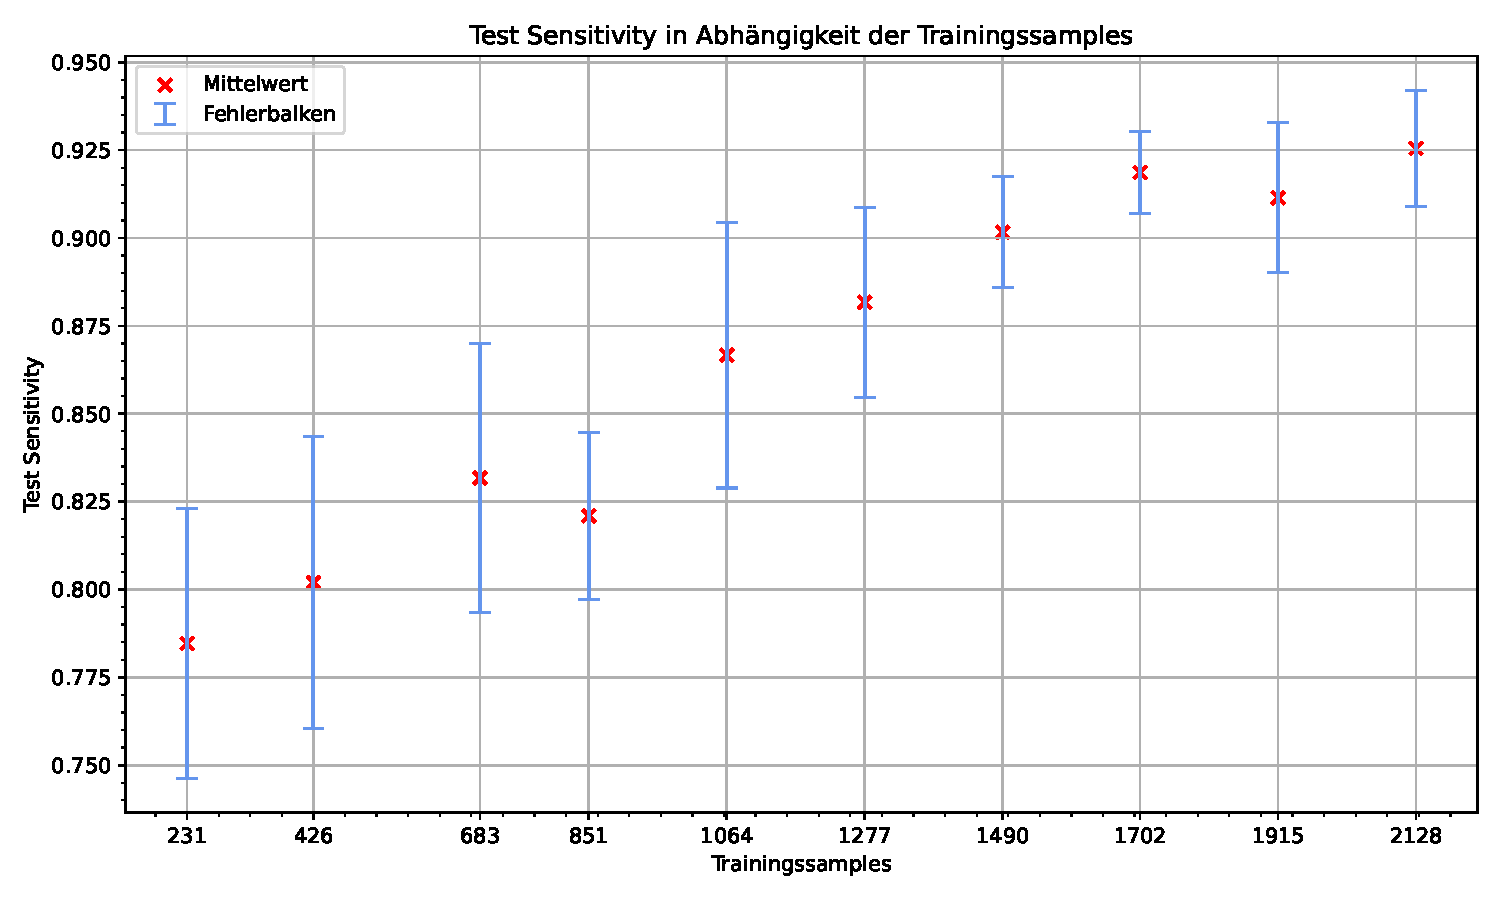
\includegraphics[width=\textwidth]{plots/3-Messungen-Gli-Men_Sensitivity_mean.pdf}
    \caption{Sensitivität}
    \label{fig:gli-men-sens}
  \end{subfigure}
  \begin{subfigure}[b]{0.48\textwidth}
    \centering
    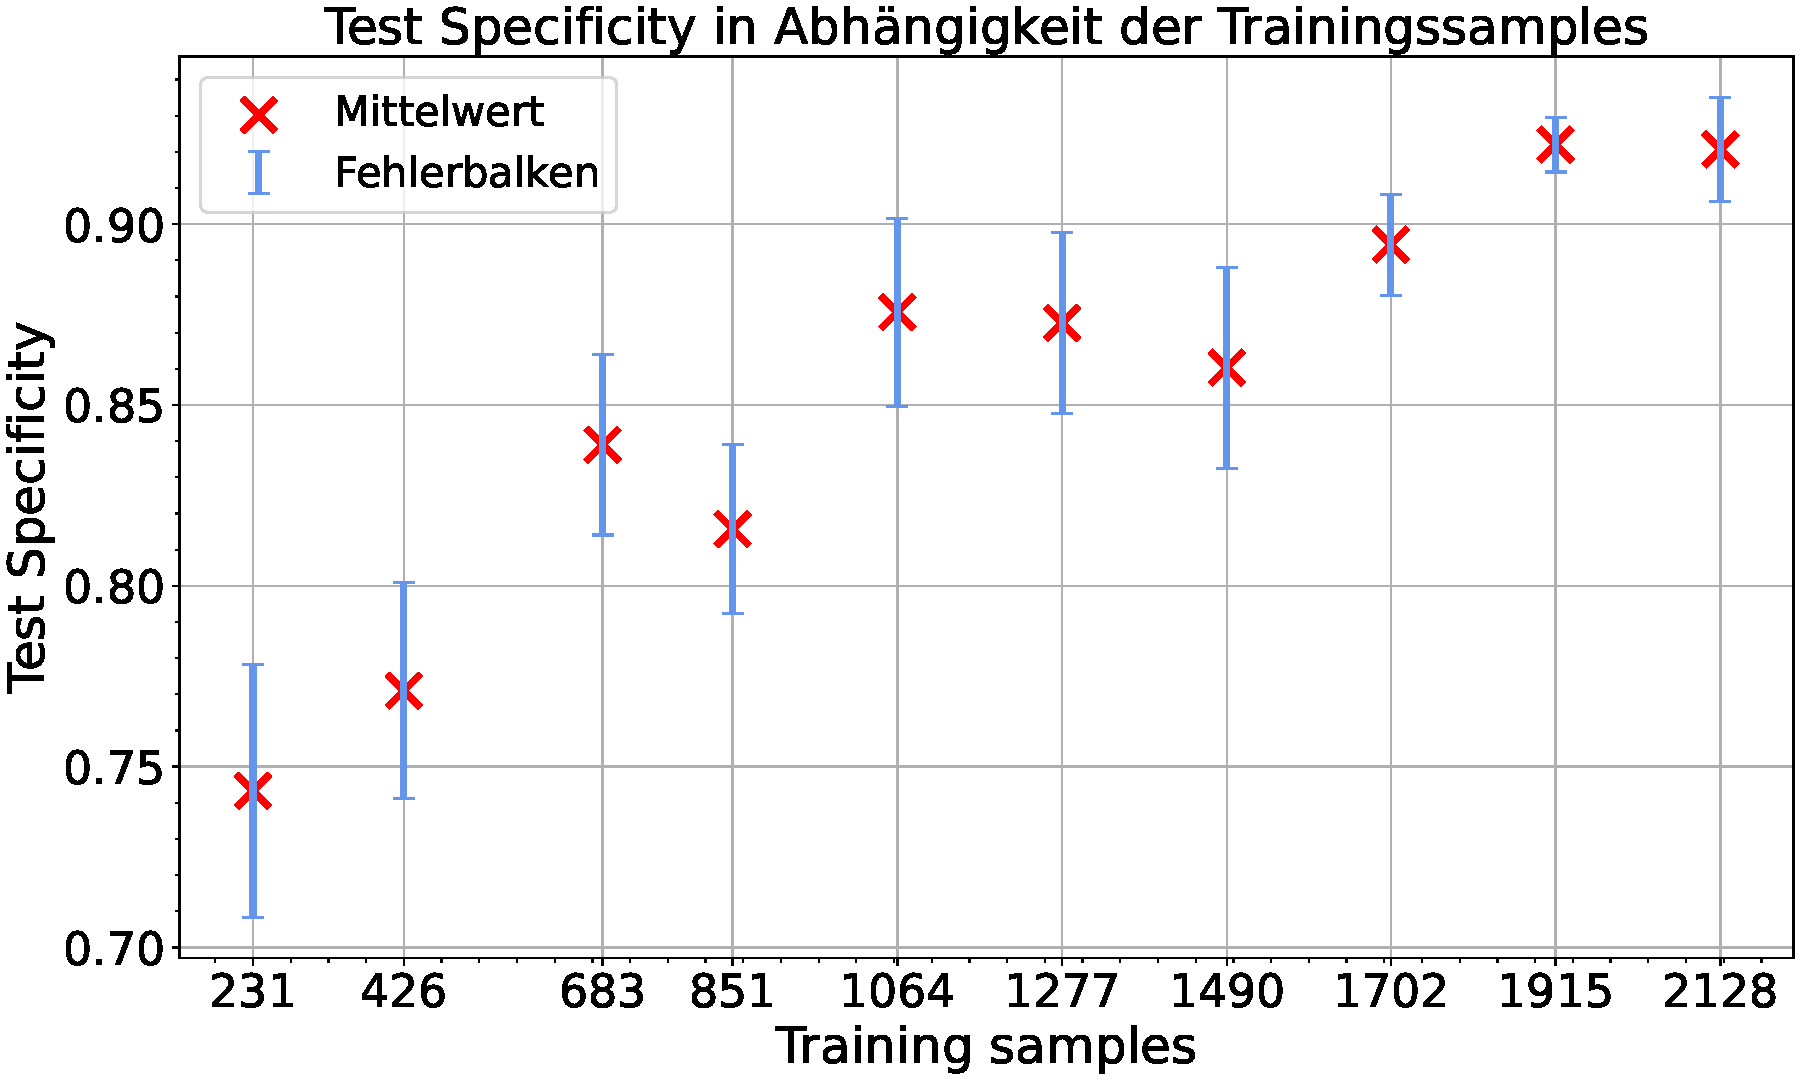
\includegraphics[width=\textwidth]{plots/3-Messungen-Gli-Men_Specificity_mean.pdf}
    \caption{Specificity}
    \label{fig:gli-men-spec}
  \end{subfigure}
  \caption{Verlauf der Metriken bei der Reduzierung der Training samples für die Klassifikation zwischen Glioma und Meningioma.}
  \label{fig:gli-men-reduktion}
\end{figure}
\begin{table}[H]
    \centering
    {\small
        \begin{tabular}{cccc}
            \toprule
            Training sample & Accuracy/$\%$ & Sensitivity & Specificity\\
            \midrule
            231  & $76.4191 \pm 0.5068$ & $0.7846 \pm 0.0383$ & $0.7433 \pm 0.0349$\\
            426  & $78.6634 \pm 0.7046$ & $0.8020 \pm 0.0414$ & $0.7710 \pm 0.0298$\\
            683  & $83.5314 \pm 1.2658$ & $0.8317 \pm 0.0383$ & $0.8390 \pm 0.0249$\\
            851  & $81.8317 \pm 1.2934$ & $0.8209 \pm 0.0238$ & $0.8157 \pm 0.0233$\\
            1064 & $87.1122 \pm 1.2506$ & $0.8667 \pm 0.0378$ & $0.8757 \pm 0.0260$\\
            1277 & $87.7228 \pm 0.6518$ & $0.8817 \pm 0.0270$ & $0.8727 \pm 0.0250$\\
            1490 & $88.1188 \pm 0.8903$ & $0.9016 \pm 0.0158$ & $0.8603 \pm 0.0278$\\
            1702 & $90.6601 \pm 0.5934$ & $0.9186 \pm 0.0117$ & $0.8943 \pm 0.0140$\\
            1915 & $91.6667 \pm 0.9212$ & $0.9114 \pm 0.0214$ & $0.9220 \pm 0.0076$\\
            2128 & $92.3102 \pm 0.8313$ & $0.9255 \pm 0.0165$ & $0.9207 \pm 0.0143$\\            
            \bottomrule
        \end{tabular}}
  \caption{Mittelwert und Standardabweichung für die Reduzierung der Training samples.}
  \label{tab:Red-gli-men}
\end{table}

\subsection{Augmentation}
Unter Verwendung von Augmentation werden die Training samples reduziert.
Der Verlauf der Metriken wird in der Abbildung \ref{fig:gli-men-augm} dargestellt.
Die dazu gehörigen Werte sind in der Tabelle \ref{tab:gli-men-augm} zu finden.

\begin{figure}[H]
  \centering
  \begin{subfigure}[b]{0.48\textwidth}
    \centering
    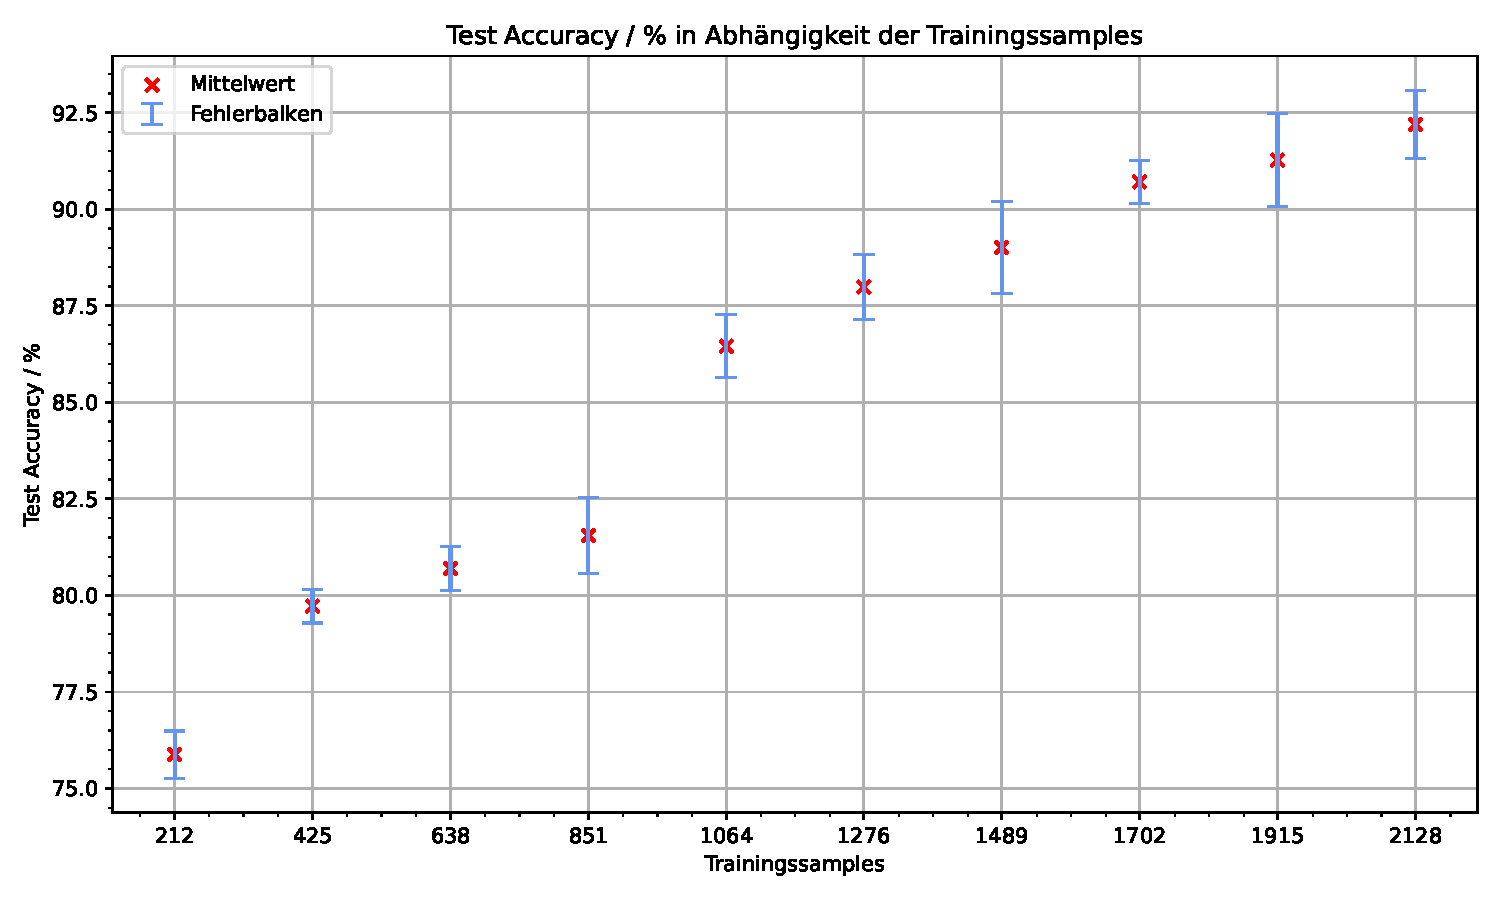
\includegraphics[width=\textwidth]{plots/Augm-Gli-Men_Accuracy_mean.pdf}
    \caption{Accuracy}
    \label{fig:augm-acc}
  \end{subfigure}
  \begin{subfigure}[b]{0.48\textwidth}
    \centering
    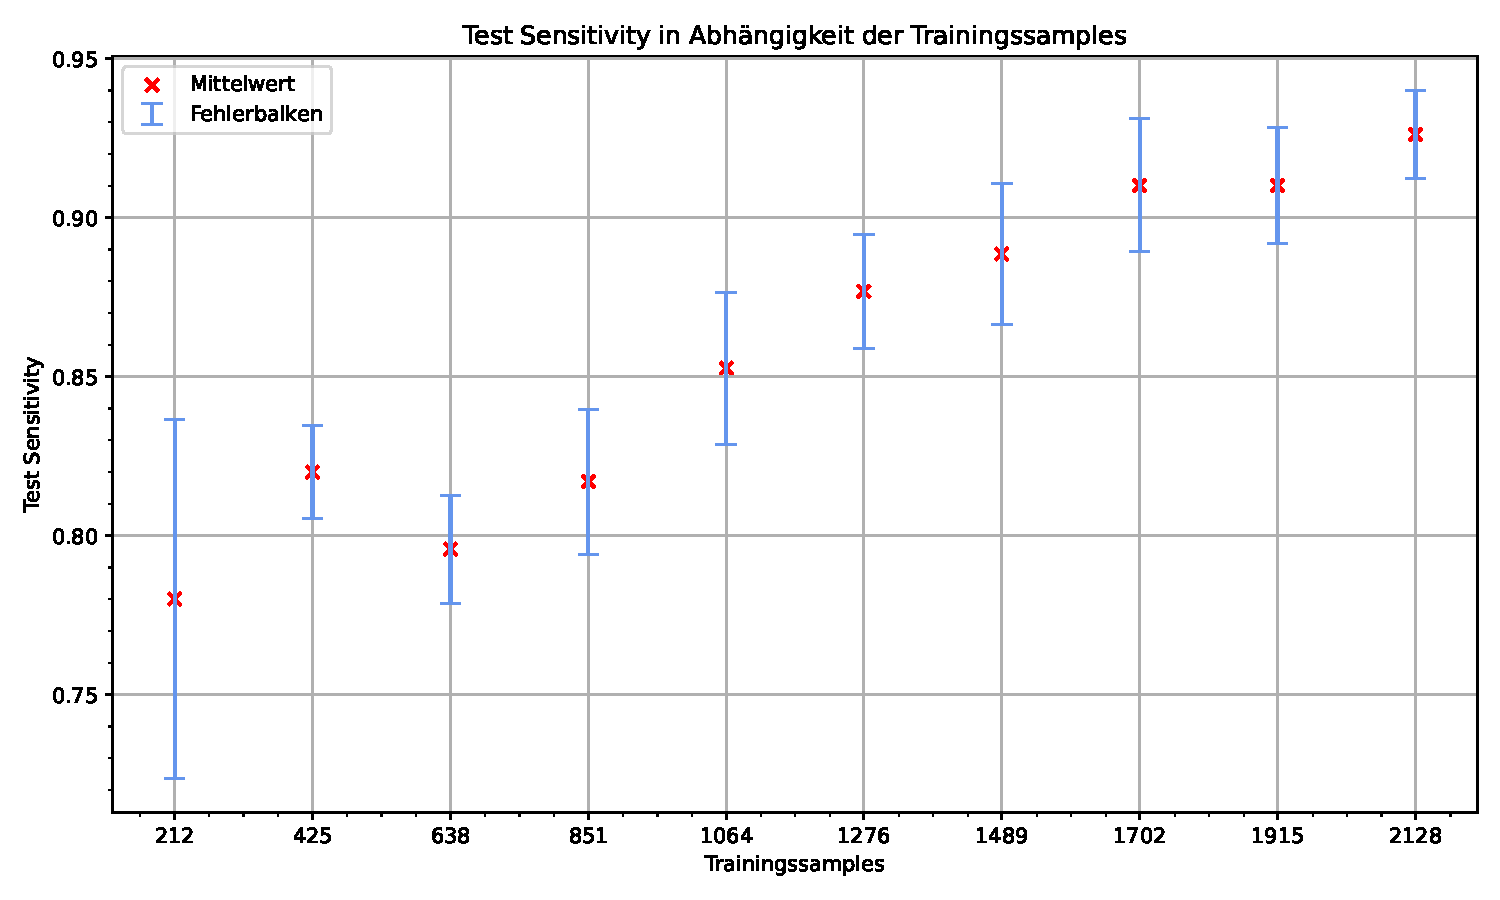
\includegraphics[width=\textwidth]{plots/Augm-Gli-Men_Sensitivity_mean.pdf}
    \caption{Sensitivität}
    \label{fig:augm-sens}
  \end{subfigure}
  \begin{subfigure}[b]{0.48\textwidth}
    \centering
    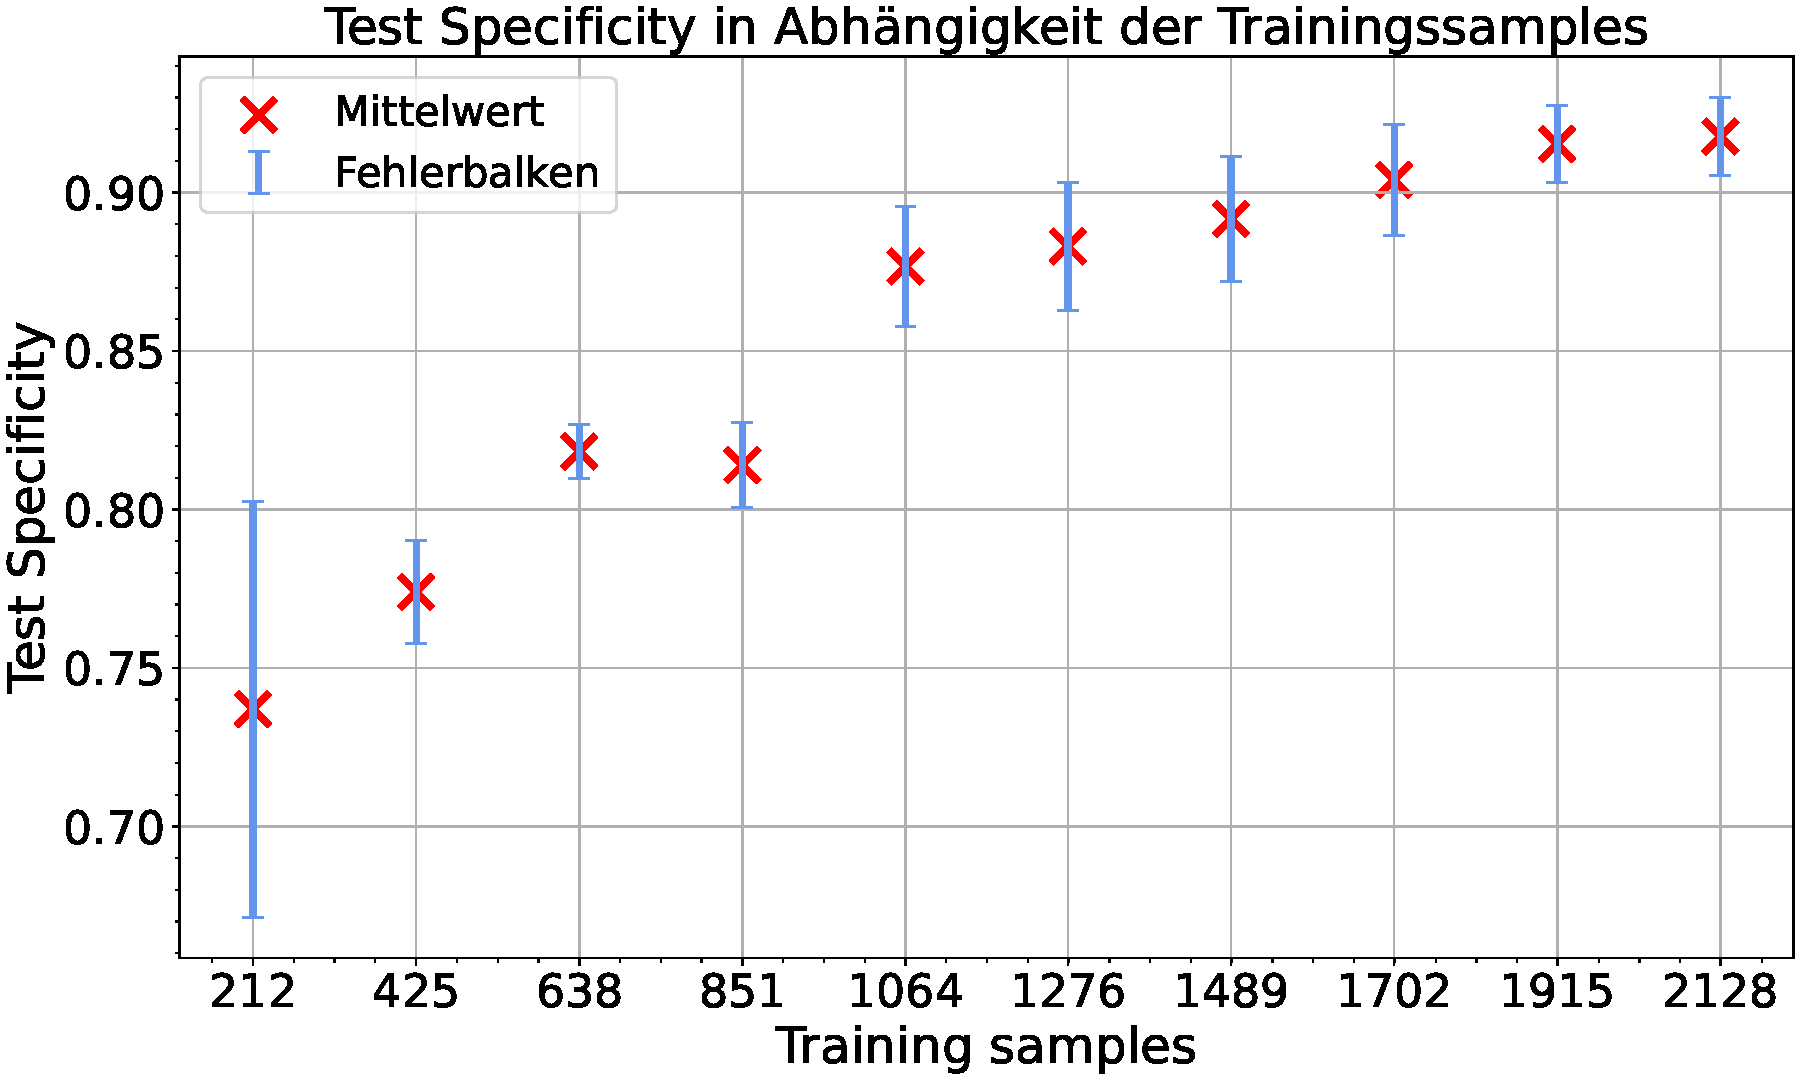
\includegraphics[width=\textwidth]{plots/Augm-Gli-Men_Specificity_mean.pdf}
    \caption{Specificity}
    \label{fig:augm-spec}
  \end{subfigure}
  \caption{Verlauf der Metriken bei Reduzierung der Training samples unter Verwendung von Augmentation für die Klassifikation zwischen Glioma und Meningioma.}
  \label{fig:gli-men-augm}
\end{figure}
\begin{table}[H]
    \centering
    {\small
        \begin{tabular}{cccc}
            \toprule
            Training sample & Accuracy/$\%$ & Sensitivity & Specificity\\
            \midrule
            212  & $75.8746 \pm 0.6115$ & $0.7801 \pm 0.0564$ & $0.7370 \pm 0.0656$ \\
            425  & $79.7195 \pm 0.4362$ & $0.8199 \pm 0.0147$ & $0.7740 \pm 0.0162$ \\
            638  & $80.6931 \pm 0.5663$ & $0.7958 \pm 0.0170$ & $0.8183 \pm 0.0085$ \\
            851  & $81.5512 \pm 0.9834$ & $0.8170 \pm 0.0228$ & $0.8140 \pm 0.0134$ \\
            1064 & $86.4521 \pm 0.8212$ & $0.8526 \pm 0.0239$ & $0.8767 \pm 0.0191$ \\
            1276 & $87.9868 \pm 0.8479$ & $0.8768 \pm 0.0180$ & $0.8830 \pm 0.0202$ \\
            1489 & $89.0099 \pm 1.1930$ & $0.8886 \pm 0.0221$ & $0.8917 \pm 0.0196$ \\
            1702 & $90.7096 \pm 0.5612$ & $0.9101 \pm 0.0209$ & $0.9040 \pm 0.0175$ \\
            1915 & $91.2706 \pm 1.2037$ & $0.9101 \pm 0.0182$ & $0.9153 \pm 0.0121$ \\
            2128 & $92.1947 \pm 0.8837$ & $0.9261 \pm 0.0139$ & $0.9177 \pm 0.0123$ \\         
            \bottomrule
        \end{tabular}}
  \caption{augm glimen}
  \label{tab:gli-men-augm}
\end{table}

\subsection{Reduzierung der Glioma sample}
\begin{figure}[H]
  \centering
  \begin{subfigure}[b]{0.48\textwidth}
    \centering
    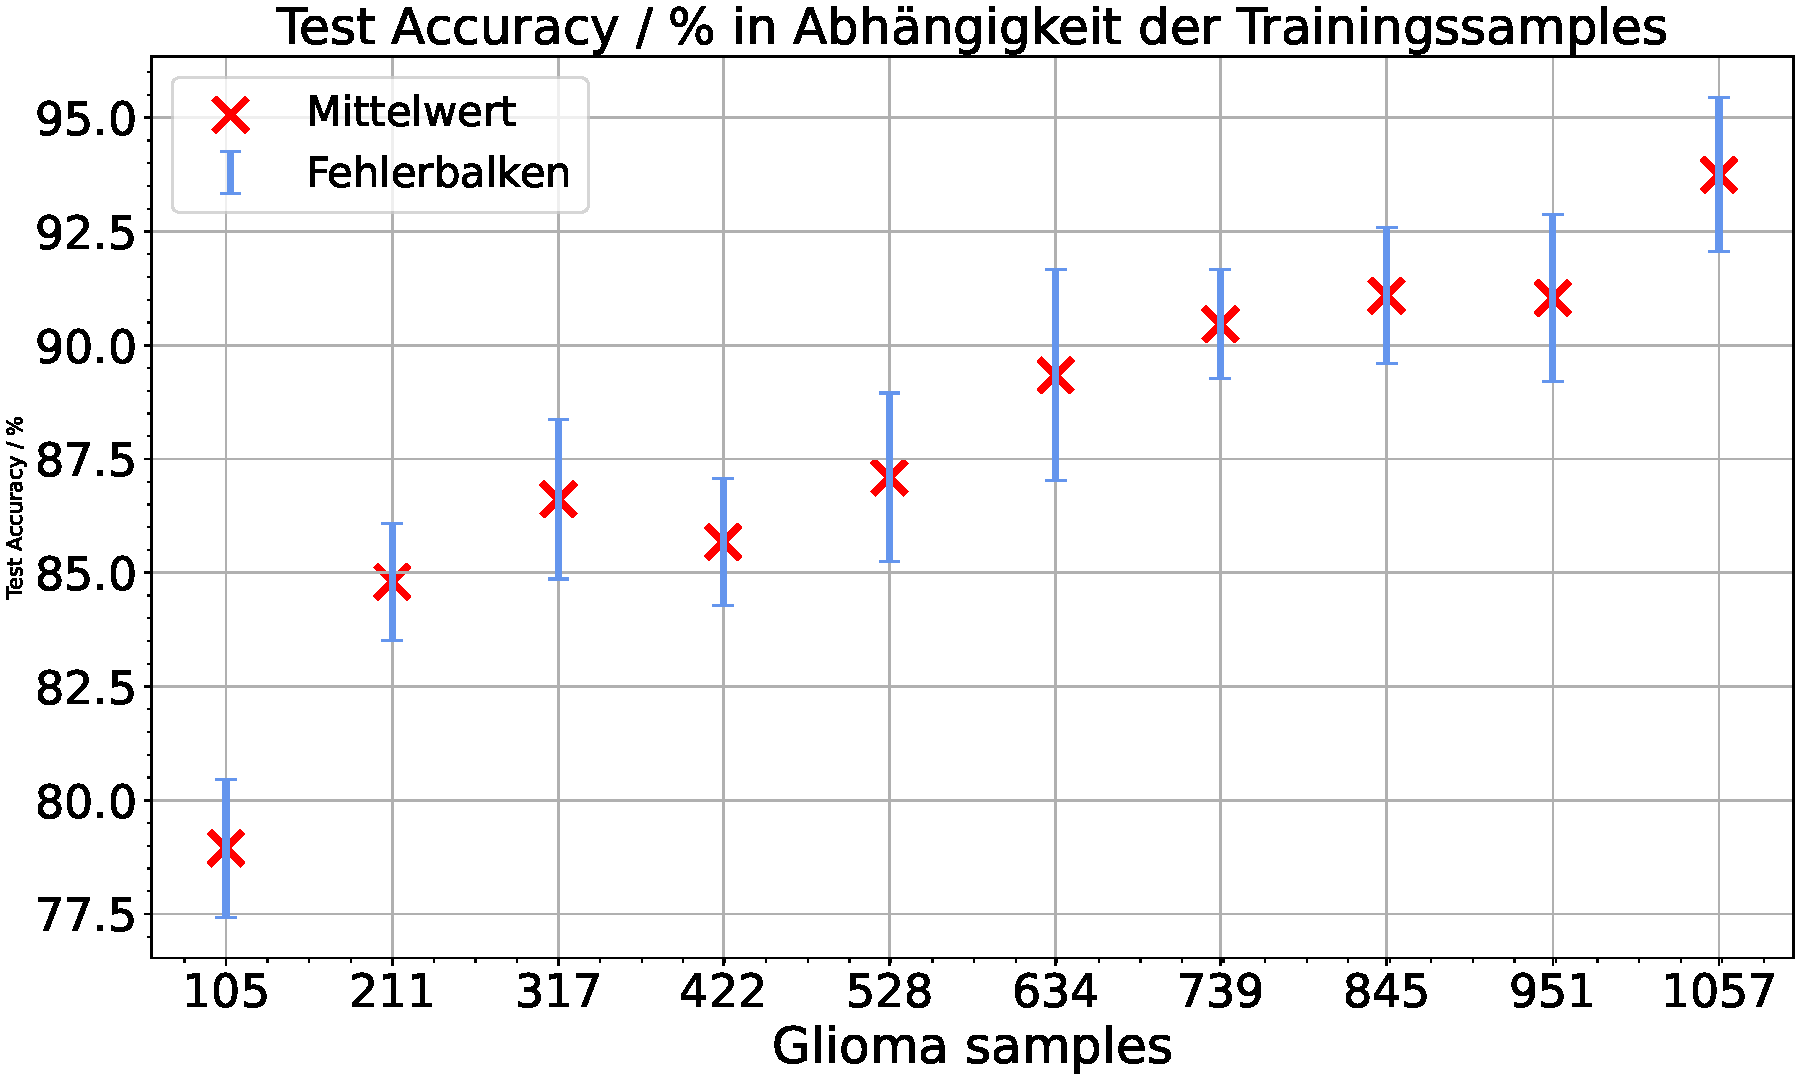
\includegraphics[width=\textwidth]{plots/Reduzierung-Gli + Balnce_Accuracy_mean.pdf}
    \caption{Accuracy}
    \label{fig:gli-red-acc}
  \end{subfigure}
  \begin{subfigure}[b]{0.48\textwidth}
    \centering
    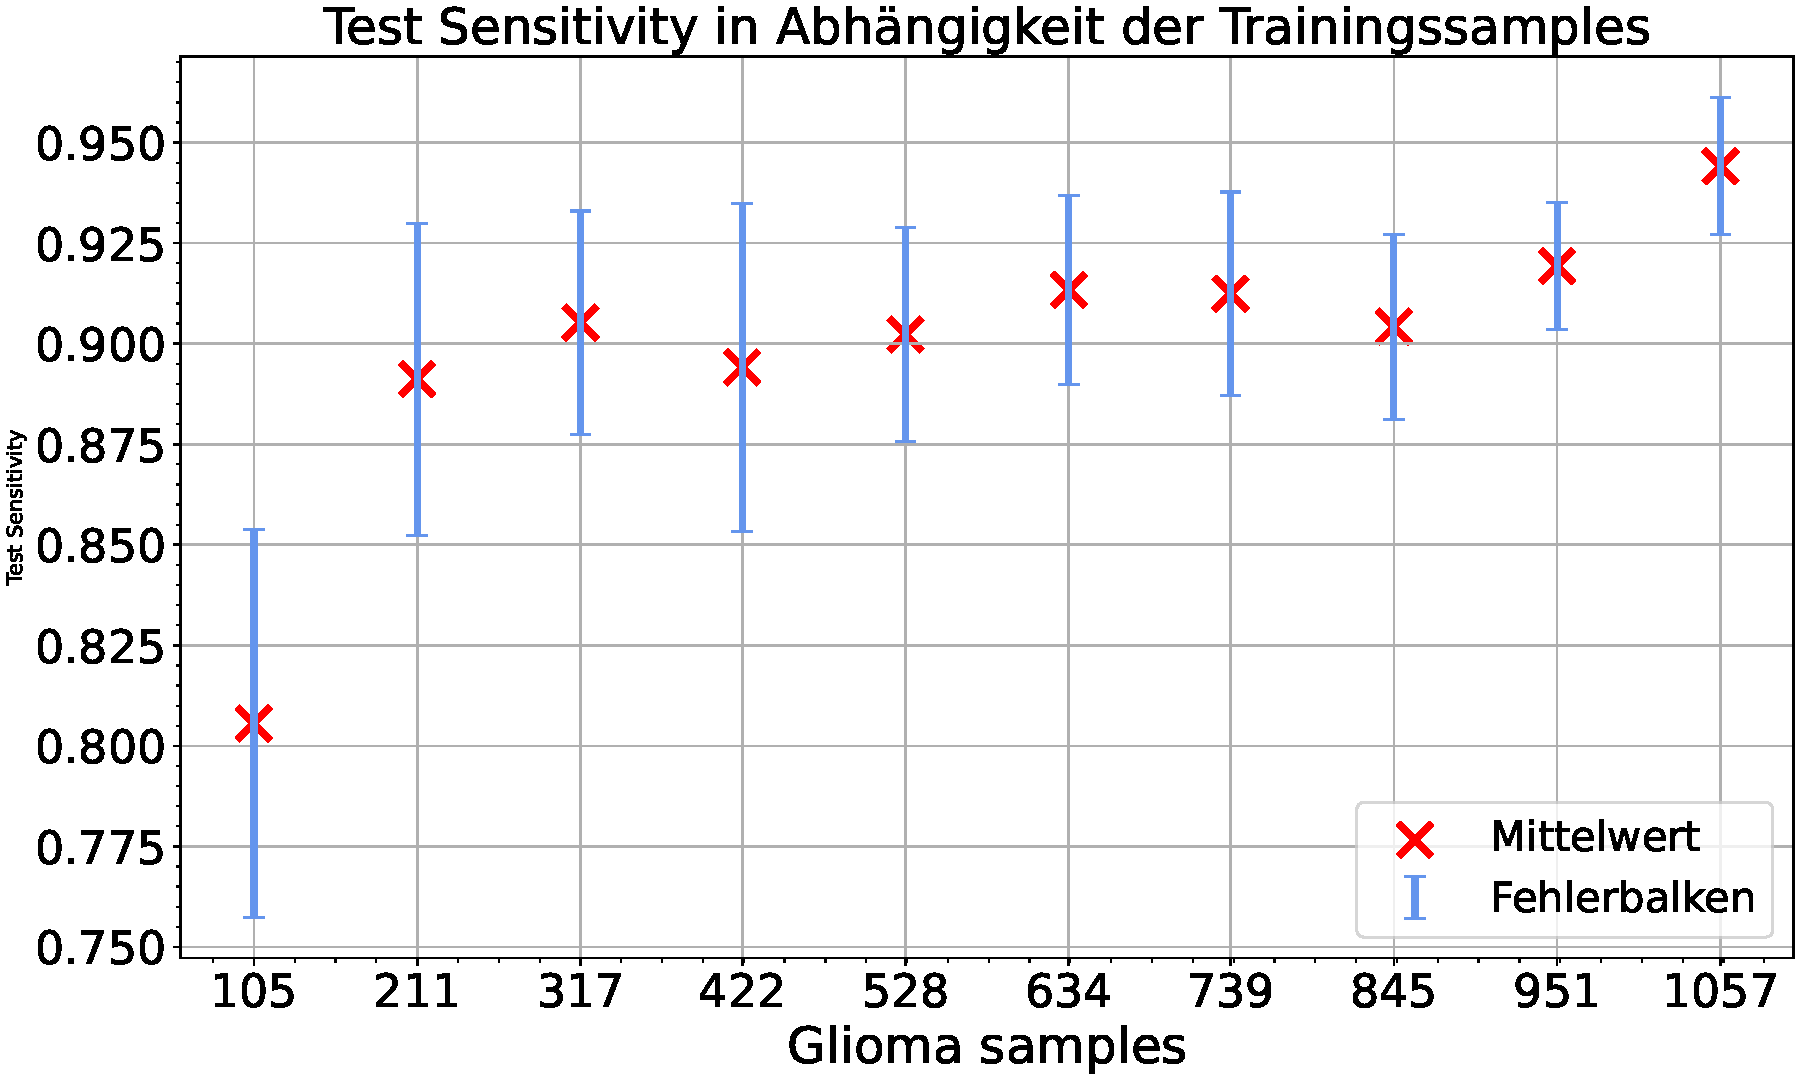
\includegraphics[width=\textwidth]{plots/Reduzierung-Gli + Balnce_Sensitivity_mean.pdf}
    \caption{Sensitivität}
    \label{fig:gli-red-sens}
  \end{subfigure}
  \begin{subfigure}[b]{0.48\textwidth}
    \centering
    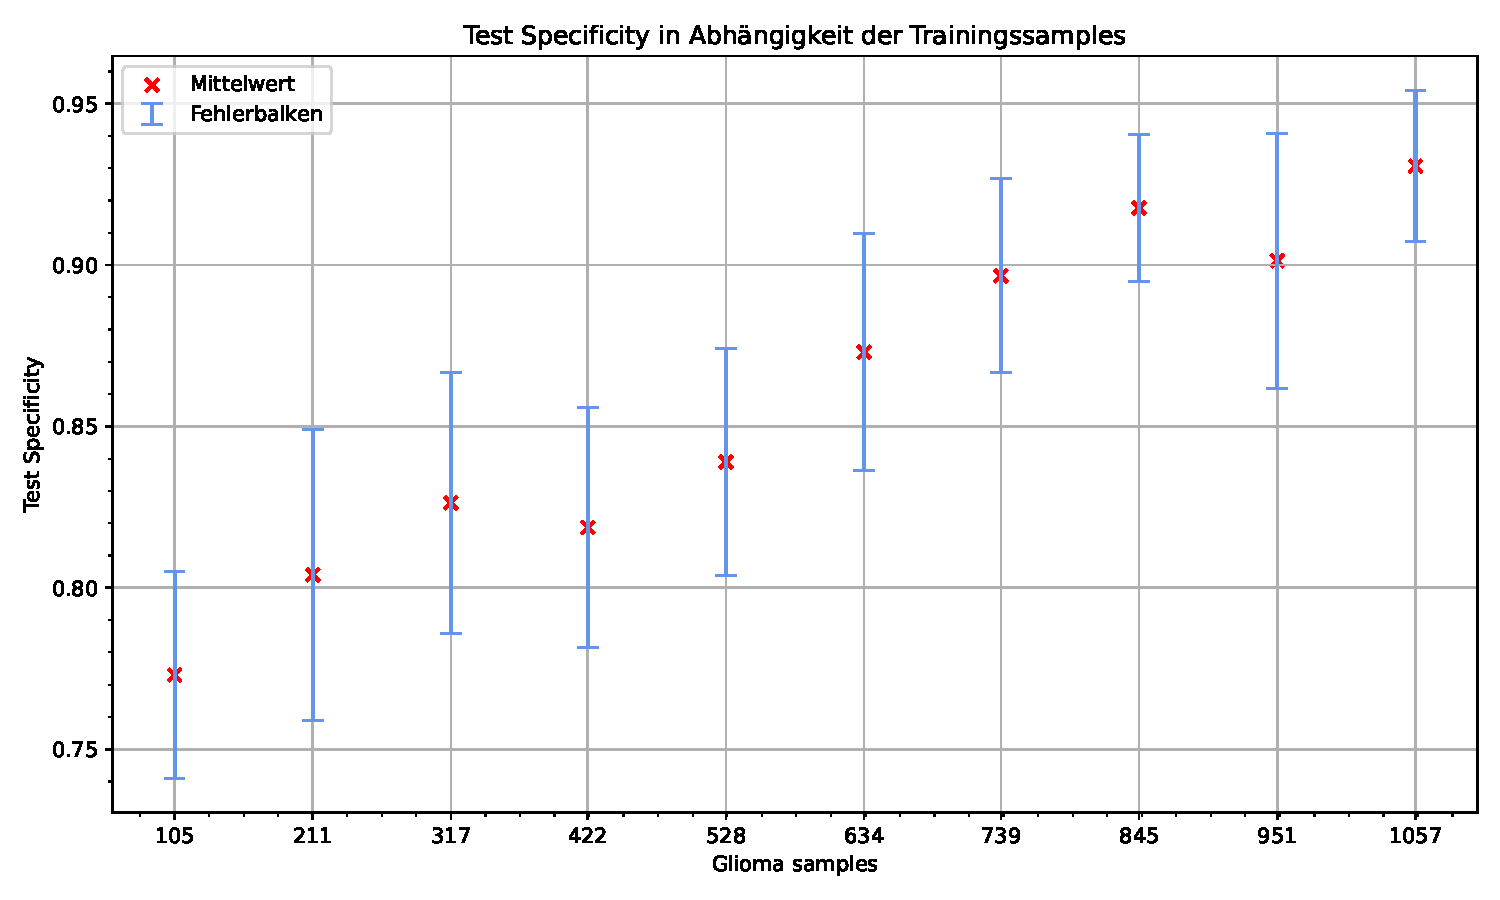
\includegraphics[width=\textwidth]{plots/Reduzierung-Gli + Balnce_Specificity_mean.pdf}
    \caption{Specificity}
    \label{fig:gli-red-spec}
  \end{subfigure}
  \caption{.}
  \label{fig:gli-men-gliored}
\end{figure}

\begin{table}[H]
    \centering
    {\small
        \begin{tabular}{cccc}
            \toprule
            Training sample & Accuracy/$\%$ & Sensitivity & Specificity\\
            \midrule
            212  & $81.8694 \pm 8.1081$ & $0.8979 \pm 0.0389$ & $0.7002 \pm 0.2544$ \\
            425  & $89.8022 \pm 1.2611$ & $0.8916 \pm 0.0179$ & $0.9077 \pm 0.0285$ \\
            638  & $90.3363 \pm 2.3230$ & $0.8959 \pm 0.0170$ & $0.9146 \pm 0.0622$ \\
            851  & $93.6696 \pm 1.1535$ & $0.9183 \pm 0.0151$ & $0.9642 \pm 0.0203$ \\
            1064 & $94.2038 \pm 0.8486$ & $0.9271 \pm 0.0156$ & $0.9644 \pm 0.0135$ \\
            1276 & $91.9189 \pm 11.273$ & $0.9441 \pm 0.0258$ & $0.8820 \pm 0.3100$ \\
            1489 & $96.1029 \pm 0.6919$ & $0.9469 \pm 0.0095$ & $0.9822 \pm 0.0118$ \\
            1702 & $96.7458 \pm 1.0820$ & $0.9512 \pm 0.0150$ & $0.9919 \pm 0.0069$ \\
            1915 & $96.6469 \pm 1.1234$ & $0.9515 \pm 0.0124$ & $0.9889 \pm 0.0111$ \\
            2128 & $92.0376 \pm 18.269$ & $0.8701 \pm 0.3058$ & $0.9956 \pm 0.0036$ \\
            \bottomrule
        \end{tabular}}
  \caption{Red Gli}
  \label{tab:}
\end{table}

